\documentclass[12pt,a4paper]{report}


\usepackage[utf8]{inputenc}
\usepackage{amsmath}
\usepackage{amsfonts}
\usepackage{amssymb}
\usepackage{graphicx}
\usepackage{amsthm}
\usepackage{natbib}
\usepackage{algorithm}
\usepackage{algpseudocode}

\usepackage{hyperref}
\AtBeginDocument{\let\textlabel\label}

\usepackage{marginnote}
\renewcommand*{\marginfont}{\scriptsize }

\usepackage{thmtools} % for lists of theorems


% Custom environments

\theoremstyle{plain}
\newtheorem{thm}{Theorem}[section]
\newtheorem{lemma}{Lemma}[section]
\newtheorem{prop}{Proposition}[section]

\theoremstyle{definition}
\newtheorem{definition}{Definition}[chapter]
\newtheorem{remark}{Remark}[section]
\newtheorem{example}{Example}[section]




% Custom commands

\newcommand{\naive}{na\"{\i}ve }
\newcommand{\Naive}{Na\"{\i}ve }
\newcommand{\andor}{and\textbackslash or }
\newcommand{\erdos}{Erd\H{o}s }
\newcommand{\renyi}{R\`enyi }


\newcommand{\al}{\alpha}
\newcommand{\be}{\beta}

\newcommand{\set}[1]{\left\{ #1 \right\}} % A set
\newcommand{\rv}[1]{\mathbf{#1}} % A random variable
\newcommand{\x}{\rv x} % The random variable x 
\newcommand{\y}{\rv y} % The random variable x 
\newcommand{\X}{\rv X} % The random variable x 
\newcommand{\Y}{\rv Y} % The random variable y
\newcommand{\expect}[1]{\mathbf{E}\left[ #1 \right]} % The expectation operator
\newcommand{\expectg}[2]{\mathbf{E}_{\rv{#1}}\left[ \rv{#2} \right]} % An expectation w.r.t. a particular random variable.
\newcommand{\expectn}[1]{\mathbb{E}\left[#1\right]} % The empirical expectation
\newcommand{\cov}[1]{\mathbf{C}ov \left[ #1 \right]} % The expectation operator
\newcommand{\covn}[1]{\mathbb{C}ov \left[ #1 \right]} % The expectation operator
\newcommand{\gauss}[1]{\mathcal{N}\left(#1\right)} % The gaussian distribution
\newcommand{\cdf}[2]{F_\rv{#1} (#2)} % The CDF function
\newcommand{\cdfn}[2]{\mathbb{F}_{#1}(#2)} % The empirical CDF function
\newcommand{\icdf}[2]{F_\rv{#1}^{-1} (#2)} % The invecrse CDF function
\newcommand{\icdfn}[2]{\mathbb{F}^{-1}_{#1}(#2)} % The inverse empirical CDF function
\newcommand{\pdf}{p} % The probability density function
\newcommand{\prob}[1]{P\left( #1 \right)} % the probability of an event
\newcommand{\dist}{P} % The proabaiblity distribution
\newcommand{\entropy}{H} % entropy
\newcommand{\mutual}[2]{I\left(#1;#2\right)} % mutual information

\newcommand{\estim}[1]{\widehat{#1}} % An estimator

\newcommand{\norm}[1]{\Vert #1 \Vert} % The norm operator
\newcommand{\normII}[1]{\norm{#1}_2} % The norm operator
\newcommand{\normI}[1]{\norm{#1}_1} % The norm operator
\newcommand{\normF}[1]{\norm{#1}_{Frob}} % The Frobenius matrix norm
\newcommand{\ones}{\textbf{1}} % Vector of ones.
\newcommand{\lik}{\mathcal{L}} % The likelihood function
\newcommand{\loglik}{L} % The log likelihood function
\newcommand{\loss}{l} % A loss function
\newcommand{\risk}{R} % The risk function
\newcommand{\riskn}{\mathbb{R}} % The empirical risk
\newcommand{\deriv}[2]{\frac{\partial #1}{\partial #2}} % A derivative
\newcommand{\argmin}[2]{\mathop{argmin} _{#1}\set{#2}} % The argmin operator
\newcommand{\argmax}[2]{\mathop{argmax}_{#1}\set{#2}} % The argmin operator
\newcommand{\hyp}{f} % A hypothesis
\newcommand{\hypclass}{\mathcal{F}} % A hypothesis class
\newcommand{\hilbert}{\mathcal{H}}
\newcommand{\rkhs}{\hilbert_\kernel} % A hypothesis class
\newcommand{\normrkhs}[1]{\norm{#1}_{\rkhs}} % the RKHS function norm


\newcommand{\plane}{\mathbb{L}} % A hypoerplane
\newcommand{\categories}{\mathcal{G}} % The categories set.
\newcommand{\positive}[1]{\left[ #1 \right]_+} % The positive part function
\newcommand{\kernel}{\mathcal{K}} % A kernel function
\newcommand{\featureS}{\mathcal{X}} % The feature space
\newcommand{\indicator}[1]{I_{\set{#1}}} % The indicator function.
\newcommand{\reals}{\mathbb{R}} % the set of real numbers



\newcommand{\latent}{\rv{s}} % latent variables matrix
\newcommand{\latentn}{S} % latent variables matrix
\newcommand{\loadings}{A} % factor loadings matrix
\newcommand{\rotation}{R}  % rotation matrix
\newcommand{\similaritys}{\mathfrak{S}} % a similarity graph
\newcommand{\similarity}{s} % A similarity measure.
\newcommand{\dissimilarity}{d} % A dissimilarity measure.
\newcommand{\dissimilaritys}{\mathfrak{D}} % a dissimilarity graph
\newcommand{\scalar}[2]{\left< #1,#2 \right>} % a scalar product



\newcommand{\manifold}{\mathcal{M}} % A manifold.
\newcommand{\project}{\hookrightarrow} % The orthogonal projection operator.
\newcommand{\projectMat}{H} % A projection matrix.
\newcommand{\rank}{q} % A subspace rank.
\newcommand{\dimy}{K} % The dimension of the output.
\newcommand{\encode}{E} % a linear encoding matrix
\newcommand{\decode}{D} % a linear decoding matrix
\DeclareMathOperator{\Tr}{Tr}
\newcommand{\ensembleSize}{M} % Size of a hypothesis ensemble.
\newcommand{\ensembleInd}{m} % Index of a hypothesis in an ensemble.


\newcommand{\sample}{\mathcal{S}} % A data sample.
\newcommand{\test}{\risk(\hyp)} % The test error (risk)
\newcommand{\train}{\riskn(\hyp)} % The train error (empirical risk)
\newcommand{\insample}{\bar{\risk}(\hyp)} % The in-sample test error.
\newcommand{\EPE}{\risk(\hat{\hyp}_n)} % The out-of-sample test error.
\newcommand{\folds}{K} % Cross validation folds 
\newcommand{\fold}{k} % Index of a fold
\newcommand{\bootstraps}{B} % Bootstrap samples
\newcommand{\bootstrap}{{b^*}} % Index of a bootstrap replication


\newcommand{\rankings}{\mathcal{R}} % Rankings, for colaborative filtering.
\newcommand{\ranking}{r} % Rankings, for colaborative filtering.
\newcommand{\kl}[2]{D_{KL}\left(#1 \Vert #2 \right)}
\newcommand{\ortho}{\mathbb{O}} % space of orthogonal matrices


\author{Jonathan Rosenblatt}
\title{Class Notes (experimental)}


\begin{document}

\maketitle

\tableofcontents





%%%%%%%%% Algorithms %%%%%%%%%%%
\newpage
\listofalgorithms
\addcontentsline{toc}{chapter}{List of Algorithms}

\renewcommand{\listtheoremname}{List of Definitions}
\listoftheorems[ignoreall,show={definition}]



\chapter{Introduction}


This text draws from \cite{hastie_elements_2003} and \cite{shalev-shwartz_understanding_2014}.
The former is freely available online.
For a softer introduction, with more hands-on examples, see \cite{james_introduction_2013}, also freely available online.
All books are very well written and strongly recommended.

The notation conventions used in this text have been collected in Appendix \ref{apx:notation}.




% % % % % Estimation % % % % %

\chapter{Estimation}
\label{sec:estimation} 

In this section, we present several estimation principles. 
Their properties are not discussed, as the section is merely a reminder and a preparation for what follows.
These concepts and examples can be found in many introductory books to statistics. I particularly recommend \cite{wasserman_all_2004} or \cite{abramovich_statistical_2013}.

\section{Moment matching}
\label{sec:moment_matching}

The fundamental idea: match empirical moments to theoretical. I.e., estimate
$$ \expect{g(X)}   $$
by 
$$ \expectn{g(X)}   $$
where $\expectn{g(x)}:=\frac{1}{n}  \sum_i g(x_i)$, is the empirical mean.

\begin{example}[Exponential Rate]

Estimate $\lambda$ in $\x_i \sim exp(\lambda)$, $i=1,\dots,n$, i.i.d.
$\expect{x}=1/\lambda$.
$\Rightarrow \estim{\lambda}=1/\expectn{x}$ .

\end{example}


\begin{example}[Linear Regression]

Estimate $\be$ in $\y \sim \gauss{X\be,\sigma^2 I}$, a $p$ dimensional random vector.
$\expect{y}=X\be$ and $\expectn{y}=y$.
Clearly, moment matching won't work because no $\be$ satisfies $X\be=y$.
A technical workaround:
Since $\be$ is $p$ dimensional, I need to find some $g(\y): \mathbb{R}^n \mapsto \mathbb{R}^p$.
Well, $g(y):=Xy$ is such a mapping. I will use it, even though my technical justification is currently unsatisfactory. We thus have:
$\expect{X'y}=X'X\be$ which I match to $\expectn{X'y}=X'y$:
$$
  X'X \be = X' y \Rightarrow \estim{\be}=(X'X)^{-1} X'y.
$$

\end{example}


\section{Quantile matching}
\label{sec:quantiles}

The fundamental idea: match empirical quantiles to theoretical. 
Denoting by $\cdf{x}{t}$ the CDF of $\x$, then $\icdf x \al$ is the $\al$ quantile of $\x$.
Also denoting by $\cdfn x t$ the Empirical CDF of $x_1,\dots, x_n$, then $\icdfn x \al$ is the $\al$ quantile of $x_1,\dots, x_n$.
The quantile matching method thus implies estimating
$$ \icdf x \al $$
by 
$$ \icdfn x \al  . $$

\begin{example}[Exponential rate]
Estimate $\lambda$ in $\x_i \sim exp(\lambda)$, $i=1,\dots,n$, i.i.d.
\begin{align*}
	& \cdf x t = 1-\exp(-\lambda t) = \al \Rightarrow \\
	& \icdf x \al = \frac{-\log(1-\al)}{\lambda} \Rightarrow \\
	& \icdf{x}{0.5} = \frac{-\log(0.5)}{\lambda} \Rightarrow \\
	& \estim{\lambda} = \frac{-\log(0.5)}{\icdfn{x}{0.5}}.
\end{align*}

\end{example}


\section{Maximum Likelihood}
\label{sec:ml}

The fundamental idea is that if the data generating process (i.e., the \emph{sampling distribution}) can be assumed, then the observations are probably some high probability instance of this process, and not a low probability event:
Let $\x_1,\dots,\x_n \sim P_\theta$, with density (or probability) $p_\theta(x_1,\dots,x_n)$.
Denote the likelihood, as a function of $\theta$: $\lik(\theta): p_\theta(x_1,\dots,x_n)$.
Then $$\estim{\theta}_{ML}:= argmax_{\theta}\set{ \lik(\theta) }.$$

Using a monotone mapping such as the log, does not change the $argmax$. 
Denote $$\loglik(\theta):=\log(\lik(\theta)).$$

 
\begin{example}[Exponential rate]

Estimate $\lambda$ in $X_i \sim exp(\lambda)$, $i=1,\dots,n$, i.i.d.
Using the exponential PDF and the i.i.d. assumption
$$ \lik(\lambda) = \lambda^n \exp(-\lambda \sum_i X_i), $$
and 
$$ \loglik(\lambda) = n \log(\lambda) -\lambda \sum_i X_i. $$

By differentiating and equating $0$, we get $\estim{\lambda}_{ML}=1/\expectn{X}$.

\end{example}

\begin{example}[Discrete time Markov Chain]

Estimate the transition probabilities,  $p_1$ and $p_2$ in a two state, $\set{0,1}$, discrete time, Markov chain where:
$P(\x_{t+1}=1|x_{t}=0)=p_1$ and $P(\x_{t+1}=1|X_{t}=1)=p_2$.
The likelihood:
$$
  \lik(p_1,p_2)=
  P(X_2,\dots,X_T;X_1,p_1,p_2)=
  \prod_{t=1}^T P(X_{t+1}=x_{t+1}|X_{t}=x_t).
$$
We denote $n_{ij}$ the total number of observed transitions from $i$ to $j$ and get that $\estim{p}_1=\frac{n_{01}}{n_{01}+n_{00}}$, and that $\estim{p}_2=\frac{n_{11}}{n_{11}+n_{10}}$.

\begin{remark}[Confession]
Well, this is a rather artificial example, as because of the Markov property, and the stationarity of the process, we only need to look at transition events, themselves Bernoulli distributed. 
This example does show, however, the power of the ML method to deal with non i.i.d. samples. As does the next example.
\end{remark}
\end{example}




\begin{example}[Autoregression of order 1 (AR(1))]
Estimate the drift parameter $a$,  in a discrete time Gaussian process where:
$\x_{t+1}=a \x_t+ \varepsilon; \varepsilon \sim \gauss{0,\sigma^2} \Rightarrow \x_{t+1}|\x_t \sim \gauss{a x_t,\sigma^2}$.

We start with the conditional density at time $t+1$:
$$
  p_{\x_{t+1}|\x_t=x_t}(x_{t+1}) = 
  (2 \pi \sigma^2)^{-1/2} \exp \left( 
    -\frac{1}{2 \sigma^2}(x_{t+1}-a x_t)^2 
  \right).
$$
Moving to the likelihood:
$$
  \lik(a) = 
  (2 \pi \sigma^2)^{-T/2} \exp \left(
    -\frac{1}{2 \sigma^2}\sum_{t=1}^T (x_{t+1}-a x_t)^2 
  \right).
$$
Taking the log and differentiating with respect to $a$ and equating $0$ we get $\estim{a}_{ML}=\frac{\sum x_{t+1}x_{t}}{\sum x_t^2}$.

We again see the power of the ML device.
Could we have arrived to this estimator by intuiton alone? Hmmmm... maybe. 
See that $Cov[X_{t+1},X_t] = a \; Var[X_t] \Rightarrow a=\frac{Cov[X_{t+1},X_t]}{Var[X_t]}$.
So $a$ can also be derived using the moment matching method which is probably more intuitive.

\end{example}




\begin{example}[Linear Regression]

Estimate $\be$ in $Y \sim \gauss{X\be,\sigma^2 I}$, a $p$ dimensional random vector.
Recalling the multivariate Gaussian PDF:
$$
  p_{\mu,\Sigma}(y) = 
  (2 \pi)^{-n/2} |\Sigma|^{-1/2} \exp\left(
    -\frac{1}{2} (y-\mu)' \Sigma^{-1} (y-\mu)
  \right)
$$
So in the regression setup:
$$
  \lik(\be)= 
  p_{\be,\sigma^2}(y) = 
  (2 \pi)^{-n/2} |\sigma^2 I|^{-1/2} \exp\left(
    -\frac{1}{2 \sigma^2} \normII{y-X\be}^2
  \right)
$$
and $\estim{\be}_{ML}$ equals 
\begin{align}
	\estim{\be}_{ML}=(X'X)^{-1} X'y.
\end{align}


\end{example}


\section{M-Estimation and Empirical Risk Minimization}
\label{sec:m_estimation}

M-Estimation, know as Empirical Risk Minimizaton (ERM) in the machine learning literature, is a very wide framework which stems from statistical desicion theory.
The underlying idea is that each realization of $\x$ incurs some loss, and we seek to find a "policy", in this case a parameter, $\theta^*$ that minimizes the average loss.
In the econometric literature, we dot not incur a loss, but rather a utility, we thus seek a policy that maximizes the average utility.

\begin{definition}[Loss Function]
The penalty for predicting $\theta$ when observing $x$: 
\begin{align}
	\loss(x;\theta).
\end{align}

\end{definition}
\begin{definition}[Risk Function]
The expected loss: 
\begin{align}
	\risk(\theta):=\expect{\loss(\x;\theta)}.
\end{align}

\end{definition}
Then the best prediction, $\theta^*$, being the minimizer of the expected risk is
\begin{align}
\label{eq:risk_min}
 \theta^*:= \argmin{\theta}{\risk(\theta)}.
\end{align}

As we do not know the distribution of $\x$, we cannot solve Eq.(\ref{eq:risk_min}), so we minimize the \emph{empirical} risk.
\begin{definition}[Empirical Risk]
The average loss in the sample: 
\begin{align}
	\riskn(\theta):=\expectn{\loss(x;\theta)}=\frac{1}{n}\sum_i \loss(x_i,\theta).
\end{align}
\end{definition}

A prediction that can actually be computed with data is thus the empirical minimizer $\estim{\theta}$:
\begin{align}
\label{eq:empirical_risk_min}
 \estim{\theta}:= \argmin{\theta}{\riskn(\theta)}.
\end{align}



\begin{example}[Squared Loss]
\label{eg:squared_loss}

Let $\loss(x;\theta)=(x-\theta)^2$. Then 
$
	\risk(\theta) = 
	\expect{(\x-\theta)^2} = 
	(\expect{\x}-\theta)^2 + Var[\x]. 
$
Clearly  $Var[\x]$ does not depend on $\theta$  so that $\risk(\theta)$ is minimized by $\theta^*=\expect{\x}$.
\textbf{We thus say that the expectation of a random variable is the minimizer of the squared loss.}

How do we estimate the population expectation? Well a natural estimator is the empirical mean, which is also the minimizer of the empirical risk $\riskn(x)$. The proof is immediate by differentiating. 
\end{example}


\begin{example}[Ordinary Least Squares (OLS)]
\label{eg:OLS}
Define the loss $\loss(y,x;\be):=\frac{1}{2}(y-x\be)^2$.
Computing the risk, $\expect{\frac{1}{2} \normII{\y-\x\be}^2}$ will require dealing with the joint distribution of $(\x,\y)$.
We don't really care about that right now. 
We merely want to see that the empirical risk minimizer, is actually the classical OLS problem. 
And well, it is (by definition actually):
\begin{align*}
	\riskn(\be)=\sum_{i=1}^n 	\frac{1}{2}(y_i-x_i\be)^2 = \frac{1}{2}\normII{y-x\be}^2.
\end{align*}
Minimization is easiest with vector derivatives, but I will stick to regular derivatives:
\begin{align*}
	\deriv{\riskn(\be)}{{\be_j}} = \sum_i \left[ (y_i-\sum_{j=1}^p x_{ij}\be_j)(-x_{ij}) \right]
\end{align*}
Equating $0$ yields $\estim{\be_j}=\frac{\sum_i y_i x_{ij}}{\sum_i x_{ij}^2}$.
Solving for all $j$'s and putting in matrix notation we get
\begin{align}
	\estim{\be}_{OLS}=(X'X)^{-1} X'y.
\end{align}

\end{example}


\section{Notes}

\subsection{Maximum Likelihood} 
Maximum likelihood estimators are a particular instance of M-estimators, if we set the loss function to be the negative log likelihood of the (true) sampling distribution.


\subsection{Choosing the Loss Function}
While by far the most popular, we do not automatically revert to minimizing a squared error loss.
There are several considerations when choosing the loss function.
Most ERM learning methods can be applied with different loss functions. 

The first consideration is computational complexity: if you choose a loss function that leads to a non-convex empirical risk, you are in trouble. There are no guarantees you will be able to find the risk minimizer in finite computing time.

The second consideration is the nature of the outcome $y$. Some loss functions are more appropriate to continuous $y$'s and some for categorical $y$'s. Typical loss functions for continuous $y$'s are the squared loss, absolute loss, and hinge loss.
Typical loss functions for categorical $y$'s are the Binomial likelihood loss (also known as the Cross Entropy, or Deviance), and the hinge loss. 

A third consideration, which is rarely given the importance it should get, is ``What is the meaning of $\theta^*$''? Or, ``What are we actually estimating''?
As we have seen in Example~\ref{eg:squared_loss}, the squared loss implies we are aiming to estimate the population mean.
What are we estimating when we use the hinge loss? The binomial loss? 
We will not discuss these matters, as we are discussing methods where these choices have already been made for us. 
When the day you start thinking of your own learning algorithms, you will need to give some thought to this question.



% % % % % % Supervised Learning % % % % % %

\chapter{Supervised Learning}
\label{sec:supervised}

\section{Supervised Learning By Empirical Risk Minimization (EMR)}
\label{sec:learning}



\subsection{Empirical Risk Minimization and Inductive Bias}
In Supervised Learning, or \emph{learning with teacher},  we want to extract the relation $y=\hyp(x)$ between attributes $x$ and some outcome $y$.
It is implicit, and essential, that the outcomes are observed. If this is not the case, see \emph{Unsupervised Learning }(\S\ref{sec:unsupervised}).
The attributes, also know as \emph{features}, or \emph{predictors}, are assumed to belong to some \emph{feature space} $\featureS$. \marginnote{Feature Space}

Unlike classical statistics, we don't care to explain the causal process relating $x$ and $y$, we just want good predictions.  The implied ERM problem is
\begin{align}
	\estim{\hyp}(x) := \argmin{\hyp}{\riskn(\hyp(x))} = \argmin{\hyp}{\frac{1}{n} \sum_i \loss(y_i - \hyp(x_i))}.
\end{align}
Alas, there are clearly infinitely many $\hyp$ for which $\riskn(\estim{\hyp}(x))=0$, in particular, all those where $\estim{\hyp}(x_i)=y_i, \forall i$.
All these $\hyp$ feel like very bad predictors, as they \emph{overfit} the observed data, at a cost of generalizability.\marginnote{Overfitting}
We formalize this intuition in Section~\ref{sec:desicion_theory}. 

We need to make sure that we do not learn overly complex predictors, which generalize poorly to new data.
Motivated by the fact that humans approach new problems equipped with their past experience, this regularization is called \emph{Inductive Bias}. \marginnote{Inductive Bias}
There are several ways to introduce this bias, which can be combined:
\begin{description}
\item[Constrained Hypothesis Classes]
We typically do not allow $\hyp$ to be ``any function'' but rather restrict it to belong to a certain class. In the machine learning terminology, $\hyp$ is a Hypothesis, and it belongs to $\hypclass$ which is the Hypothesis Class.\marginnote{Hypothesis}
\item[Regularization] We do not need to treat all $\hyp \in \hypclass$ equivalently. We might have prior preferences towards particular $\hyp$'s , typically simple $\hyp$'s, and we can introduce these preferences in the learning process. This is called \emph{Regularization}.\marginnote{Regularization}
\item[Non ERM Approaches] Many learning problems can be cast as ERM problems, but another way to introduce bias is by learning $\hyp$ in a non-optimal manner. Inductive bias is thus introduced by the (non) optimization algorithm 
Learning algorithms that cannot be cast as ERMs include: Nearest Neighbour (\S\ref{sec:knn}), Kernel Regression(\S\ref{sec:kernel}), Boosting (\S\ref{sec:boosting}).
\end{description}

We now proceed to show that many supervised learning algorithms are in fact ERMs with some type of inductive bias: constrained hypothesis class \andor or regularization \andor suboptimality.

\subsection{Ordinary Least Squares (OLS)}
\label{sec:ols}
As seen in Example~\ref{eg:OLS}, by adopting a squared error loss, and restricting $\hypclass$ by assuming $\hyp$ is a linear function of $x$, we get the OLS problem.
In this case learning $\hyp$ is effectively the same as learning $\be$ as they are isomorphic, as will be the case in all hypothesis classes that admit a finite dimensional parametrization.

\paragraph{Regularization}
While the OLS problem seemingly has no regularization parameters, we are in no way restricted to the original $X$ matrix supplied to us. 
We are free to choose any subset of the $X$ variables. Selecting a subset of the $X$ variables is known as \emph{model selection}.\marginnote{Model Selection}
We will discuss many different methods to choose the regularization level, in this case, the variables in the OLS, in Section~\ref{sec:desicion_theory}.

We are not only free to select a subset of $X$s, but we can also augment $X$ with new variables, consisting of non linear transformation of the original ones. This is know as \emph{basis augmentation}. \marginnote{Basis Augmentation}
The idea of basis augmentation is a useful and fundamental one that will revisit us throughout the course, even if we typically don't call it by its name.

\begin{remark}[No Sampling Distribution]
We emphasize, that unlike the classical statistical literature, we never assumed any sampling distribution. 
This is why we will not be doing hypothesis testing on the model parameters.
ERM can be thus seen as \emph{exploratory} statistics. 

In particular, we are not discussing hypothesis testing and confidence intervals for the OLS problem, for this same reason: because we are not assuming the data generating distribution. This, in contrast to the classical statistical literature where the linear model is both the data generating process, and the assume hypothesis class. 

In statistical terminology, we may be fitting \emph{misspecified models}, we simply do not care about it, as long as predictions are good. \marginnote{Misspecified Model}
\end{remark}


\begin{remark}[OLS Extensions]
Most if not all extensions of OLS, such as Generalized Least Squared (GLS) and Generalized Linear Models (\S\ref{sec:logistic}) are ERM problems. 
\end{remark}




\subsection{Ridge Regression}
\label{sec:ridge}

Consider the Ridge regression problem:
\begin{align}
\label{eq:ridge}
	& \argmin{\be}{\frac{1}{n}\sum_i (y_i-x_i\be)^2 + \frac{\lambda}{2}\normII{\be}^2} \\
	& \estim{\be}_{Ridge}= (X'X+\lambda I)^{-1} X'y
\end{align}
We can see that again, $\hypclass$ is restricted to be the space of linear functions of $x$, but we also add a regularization that favours linear functions with small coefficients.

The regularization of $\be$ can have several interpretations and justifications:
\begin{description}
\item[A mathematical device] Strengthening the diagonal of $X'X$ makes is more easily invertible. This is a standard tool in applied mathematics called \emph{Tikhonov Regularization}. It is also helpful when dealing with multicolinearity, as $(X'X+\lambda I)$ is always invertible.
\item[A Subjective Bayesian View] If we believe that $\be$ should be small; say our beliefs can be quantified by $\rv \be \sim \gauss{0,1/\lambda I}$, then the Ridge solution is actually the mean of our posterior beliefs on $\rv \be|y$.
\end{description}

Whatever justification you prefer, it can be easily shown that $\deriv{\risk(\lambda,\be)}{\lambda}$ at $\lambda=0$ is negative, thus, predictions only improve by introducing some small regularization (how small is small? See \S\ref{sec:desicion_theory}).

For more on Ridge regression see \cite{hastie_elements_2003}.


\subsection{LASSO}
\label{sec:lasso}

Consider the LASSO problem:
\begin{align}
\label{eq:lasso}
	& \argmin{\be}{\frac{1}{n}\sum_i (y_i-x_i\be)^2 + \lambda \normI{\be}} 
\end{align}
As can be seen, just like in Ridge regression, $\hypclass$ is restricted to linear functions of $x$. The regularization however differs. Instead of $l_2$ norm penalty, we use an $l_1$ norm penalty.
Eq.(\ref{eq:lasso}) does not have a closed form solution for $\estim{\be}_{LASSO}$ but the LARS algorithm, a quadratic programming algorithm, solves it efficiently.



The LASSO has gained much popularity as it has the property that $\estim{\be}_{LASSO}$ has many zero entries. It is thus said to be \emph{sparse}\marginnote{Sparsity}.
The sparsity property is very attractive as it acts as a model selection method, allowing to consider $X$s where $p>n$, and making predictions computationally efficient.

The sparsity property can be demonstrated analytically for the orthogonal design case ($X'X=I$), in which $\estim{\be}$ admits a closed form solution:
\begin{align}
	\estim{\be}_{j,LASSO} = sign(\estim{\be}_{j,OLS}) \left[|\estim{\be}_{j,OLS}|-\frac{\lambda}{2} \right]_+.
\end{align}
We thus see that the LASSO actually performs \emph{soft thresholding} on the OLS estimates. \marginnote{Soft Thresholding}




\subsection{Logistic Regression}
\label{sec:logistic}
The logistic regression is the first categorical prediction problem we consider. \marginnote{Categorical Prediction}
I.e., the outcome $y$ is not a continuous variable, but rather takes values in some finite set $\categories$. In the logistic regression problem, it can take two possible values.
In the statistical literature, $y$ is encoded as $\categories=\set{0,1}$ and $\hyp$ is assumed to take to take the following form:
\begin{align}
	& p(x):= P(\y=1|x) = \Psi(x\be) \\
	& \Psi(t) = \frac{1}{1+e^{-t}}
\end{align}
The hypothesis class is thus  $\hypclass=\set{\hyp:\hyp(x)=\Psi(x\be)} $.

In the $\set{0,1}$ encoding, the loss is the negative log likelihood, i.e.:
\begin{align}
	\loss(y,x,\be) = 
	-\log \left[ p(x)^{y} (1-p(x))^{1-y}  \right] =
	-\log \left[ \Psi(x\be)^{y} (1-\Psi(x\be))^{1-y}  \right].
\end{align}
In the learning literature it is more common for $\categories=\set{1,-1}$ encoding of $y$ in which case the loss is 
\begin{align}
	\loss(y,x,\be) = -\log \left[ 1+\exp(-y f(x))  \right].
\end{align}


\paragraph{How to classify?}
In the $\set{0,1}$ encoding, we predict class $1$ if $\Psi(x\be)>0.5$ and class $0$ otherwise.
The logistic problem thus defines a separating hyperplane $\plane \subset \featureS$ between the classes: $\plane=\set{x:f(x)=0.5}$.

In the $\set{1,-1}$ encoding, we predict class $1$ if $\Psi(x\be)>0$ and class $0$ otherwise.
The plane $\plane$ is clearly invariant to the encoding of $y$.




\begin{remark}[Generalized Linear Models (GLM)]
Logistic regression is a particular instance of the very developped theory of Generalized Linear Models.\marginnote{GLM}
These models include the OLS, Probit Regression, Poisson Regression, Quasi Likelihood, Multinomial Regression, Proportional Odds regression and more.
The ultimate reference on the matter is \cite{mccullagh_generalized_1989}.
\end{remark}




\subsection{Regression Classifier}
\label{sec:regression_classifier}
Can we use the OLS framework for prediction? Yes! With proper encoding of $y$.
Solving the same problem from Example~\ref{eg:OLS} by encoding $y$ as $\set{0,1}$ gives us the linear separating hyperplane $\plane= \set{x:x\estim{\be}_{OLS}=0.5}$.

\begin{remark}
We can interpret $\estim{y}$ as the probability of an event, but there a slight technical difficulty as $\estim{y}$ might actually be smaller than $0$ or larger than $1$.
\end{remark}




\subsection{Linear Support Vector Machines (SVM)}
\label{sec:svm}

The literature typically presents the SVM method using the geometrical arguments that originally motivated the problem. 
For our purposes, we present the ERM formulation of the problem, followed by the original arguments.
Assuming a linear hypothesis class, $\hyp(x)=\be_0+\be x$, and $\categories=\set{-1,1}$ encoding, the SVM ERM problem is

\begin{align}
\label{eq:svc_ERM}
	\min_{\be,\be_0} \set{
		\sum_i \positive{1-y_i \hyp(x_i)} +\frac{\lambda}{2} \normII{\be}^2
	}.
\end{align}
Eq.(\ref{eq:svc_ERM}) thus reveals that the linear SVM is actually an ERM problem, over a linear hypothesis class, with what is called the \emph{hinge} loss function and $l_2$ regularization of $\be$.


\subsubsection{Geometrical Motivation for SVM}
For completeness, we present Vapnik's original geometric motivation \citep{vapnik_statistical_1998} for the formulation of the SVM problem. 

We do not assume anything on the data, and seek for a hyperplane $\plane$ that seperates two classes. 
Encode $y$ as $\categories=\set{-1,1}$.
Define a plane $\plane=\set{x: \hyp(x)=0 }$, and assume a linear hypothesis class, $\hyp(x)=x\be+\be_0$.
Now find the plane $\plane$ that maximizes the (sum of) distances to the data points.
We call the minimal distance from $\plane$ to the data points, the \emph{Margin}, and denote it by $M$.

To state the optimization problem, we need to note that $\hyp(x)=x\be+\be_0$ is not only the value of our classifier, but it is actually proportional to the signed distance of $x$ from $\plane$. 
\begin{proof}
The distance of $x$ to $\plane$ is defined as $\min_{x_0 \in \plane} \set{ \normII{x-x_0} }$.
Note $\be^*:=\be/\normII{\be}$ is a normal vector to $\plane$, since $\plane=\set{x: x\be+\be_0=0 }$, so that for $x_1,x_2 \in \plane \Rightarrow \be(x_1-x_2)=0$.
Now $x-x_0$ is orthogonal to $\plane$ because $x_0$ is, by definition, the orthogonal projection of $x$ onto $\plane$.
Since $x-x_0$ are both orthogonal to $\plane$, they are linearly dependent, so that by the Cauchy Schwarz inequality $\normII{\be^*} \normII{x-x_0}= \normII{\be^*(x-x_0)}$.
Now recalling that $\normII{\be^*}=1$ and $\be^* x_0=-\be_0/\normII{\be}$ we have $\normII{x-x_0}=\frac{1}{\normII{\be}} (x\be+\be_0)= \frac{1}{\normII{\be}} \hyp(x)$.
\end{proof}

Using this fact, then $y_i \hyp(x_i)$ is the distance from $\plane$ to point $i$, positive for correct classifications and negative for incorrect classification. 
The (linear) support vector classifier is defined as the solution to
\begin{align}
\label{eq:svc_separable}
	\max_{\be,\be_0} \set{ 
		M \quad s.t. \quad 
		\forall i: y_i \hyp(x_i) \geq M, \quad \normII{\be}=1
	}
\end{align}

If the data is not separable by a plane, which is typically the case, we need to allow some slack.
We thus replace $y_i \hyp(x_i) \geq M$ with $y_i \hyp(x_i) \geq M(1-\xi_i)$, for $\xi_i>0$ but require that the missclassifications are controlled using a regularization parameter $C$: $\sum_i \xi_i \leq C$.
Eq.(\ref{eq:svc_separable}) now becomes \citep[Eq.(12.25)]{hastie_elements_2003}
\begin{align}
\label{eq:svc_non_separable}
	\max_{\be,\be_0} \set{ 
		M \quad s.t. \quad 
		\forall i: y_i \hyp(x_i) \geq M(1-\xi_i), 
		\: \normII{\be}=1, 
		\: \sum_i \xi_i \leq C,
		\:\forall i:\xi_i\ \geq 0
	}
\end{align}


See Section 12 in \cite{hastie_elements_2003} for more details on SVMs.


\begin{remark}[Name Origins]
SVM takes its name from the fact that $\estim{\be}_{SVM}=\sum_i \estim{\al}_i y_i x_i$.
The explicit form of $\estim{\al}_i$ can be found in \citep[Section 12.2.1]{hastie_elements_2003}.
For our purpose, it suffices to note that $\estim{\al}_i$ will be $0$ for all data points far away from $\plane$.
The data points for which $\estim{\al}_i>0$ are the \emph{support vectors}, which give the method its name.
\end{remark}





\begin{remark}[Solve the right problem]
Comparing with the logistic regression, and the linear classifier, we see that the SVM cares only about the decision boundary $\plane$. Indeed, if only interested in \emph{predictions}, estimating \emph{probabilities} is a needless complication. As Put by Vapnik: 
\begin{quote}
When solving a given problem, try to avoid a more general problem as an intermediate
step.
\end{quote}
Then again, if the assumed logistic model of the logistic regression, is actually a good approximation of reality, then it will outperform the SVM as it borrows information from all of the data, and not only the support vectors. 
\end{remark}


\subsection{Generalized Additive Models (GAMs)}
\label{sec:gam}
A way to allow for a more broad hypothesis calss $\hypclass$, that is still not too broad, so that overfitting is hopefully under control, is by allowing the predictor to be an additive combination of simple functions.
We thus allow $\hyp(x)=\be_0 + \sum_{j=1}^p f_j(x_j)$. We also not assume the exact form of $\set{f_j}_{j=1}^p$ but rather learn them from the data, while constraining them to take some simple form.
The ERM problem of GAMs is thus
\begin{align}
\label{eq:GAM}
	 \argmin{\hyp \in \hypclass}{\frac{1}{n}\sum_i (y_i-\hyp(x_i))^2  }
\end{align}
where $\hyp$ is as defined above.

\begin{remark}[Not a pure ERM]
The learning of $\set{f_j}_{j=1}^p$ is in fact not performed by optimization, but rather by kernel smoothing (\S~\ref{sec:kernel}).
The solution to Eq.(\ref{eq:GAM}) is not a pure ERM problem, but a hybrid between ERM and kernel smoothing.
\end{remark}



\subsection{Projection Pursuit Regression (PPR)}
\label{sec:ppr}
Another way to generalize the hypothesis class $\hypclass$, which generalizes the GAM model, is to allow $\hyp$ to be some simple function of a linear combination of the predictors. Let 
\begin{align}
\label{eq:PPR}
	\hyp(x)=\sum_{m=1}^M g_m(w_m x)
\end{align}
where both $\set{g_m}_{m=1}^M$ and $\set{w_m}_{m=1}^M$ are learned from the data. 
The regularization is now performed by choosing $M$ and the class of $\set{g_m}_{m=1}^M$.
The ERM problem is the same as in Eq.(\ref{eq:GAM}), with the appropriate $\hyp$.

\begin{remark}[Not a pure ERM]
Just like the GAM problem, in the PPR problem $\set{g_m}_{m=1}^M$ are learned by Kernel Regresson (\S\ref{sec:kernel}). Solving the PPR problem is thus a hybrid of ERM and Kernel Regresson algorithms.
\end{remark}

\begin{remark}[Universal Approximator]
By choosing a sufficiently large $M$, the class $\hypclass$ can approximate any continuous function. This property of the class is called a \emph{Universal Approximator}.\marginnote{Universal Approximator}
\end{remark}




\subsection{Neural Networks (NNETs)}
\subsubsection{Single Hidden Layer}
In the spirit of \cite[Section 11]{hastie_elements_2003}, we introduce the NNET model via the PPR model, and not through its historically original construction.
In the language of Eq.(\ref{eq:PPR}), a \emph{single-layer--feed-forward }neural network, is a model where $\set{g_m}_{m=1}^M$  are not learned from the data, but rather assumed a-priori. 
\begin{align*}
	g_m(x):= \be_m \sigma( x \al_m  )
\end{align*}
where only $\set{\be_m, \al_m}_{m=1}^M$ are learned from the data. 
A typical \emph{activation function}\marginnote{Activation Function}, $\sigma(t)$ is the standard logistic CDF: $\sigma(t)=\frac{1}{1+e^{-t}}$. Another popular alternative are Gaussian radial functions.

As can be seen, the NNET is merely a non-linear regression model.
The parameters of which are often called \emph{weights}.

NNETs have gained tremendous popularity, as they strike a good balance between model complexity and regularity; particularly in the machine vision, sound analysis and natural language processing domains, where data samples are abundant.

\paragraph{Loss Functions}
Like any other ERM problem, we are free to choose the appropriate loss function.
For regression the squared loss is used. For classification, one can still use the squared error (as in the Regression Classifier), or the binomial likelihood leading to what is know as the \emph{deviance}, or \emph{cross-entropy} loss.\marginnote{Deviance \& Cross Entropy}

\paragraph{Universal Approximator}
Like the PPR, even when $\set{g_m}_{m=1}^M$ are fixed beforehand, the class is still a universal approximator (although it might require a larger $M$ than PPR).

\paragraph{Regularization}
Regularization of the model is done via the selection of the $\sigma$, the number of nodes/variables in the network and the number of layers. More that one hidden layer leads to \emph{Deep Neural Networks} which offer even more flexibility at the cost of complexity, thus requiring many data samples for fitting.\marginnote{Deep Neural Networks}

\paragraph{Back Propagation}
The fitting of such models is done via a coordinate-wise gradient descent algorithm called \emph{back propagation}.

\paragraph{Further Reading}
For more on NNETs see \citep[Chapter 11]{hastie_elements_2003}.
For a recent overview of Deep Learning in Neural Networks see \cite{schmidhuber_deep_2015}.




\subsection{Classification and Regression Trees (CARTs)}
CARTs are a type of ERM where $\hyp(x)$ include very non smooth functions that can be interpreted as "if-then" rules, also know as \emph{decision trees}.\marginnote{Decision Tree}

The hypothesis class of CARTs includes functions of the form
\begin{align}
\label{eq:decision_list}
	\hyp(x)=\sum_{m=1}^M c_m \indicator{x \in R_m}
\end{align}
where $I_A$ is the indicator function of the event $A$.
The parameters of the model are the different conditions $\set{R_m}_{m=1}^M$ and the function's value at each condition $\set{c_m}_{m=1}^M$. 

Regularization is done by the choice of $M$ which is called the \emph{tree depth}.\marginnote{Tree Depth}

As $\hyp(x)$ is defined over indicator functions, CARTs have no difficulty to deal with categorical variables and even missing values, on top of the more standard continuous predictors. More on the many advantages of CARTs can be found in the references.

\paragraph{Optimization}
As searching over all possible partitions of the $x$'s to optimize $\set{R_m}_{m=1}^M$ is computationally impossible, optimization is done is a greedy fashion, by splitting on each variable $x_j$ at a time.
The problem presented in Eq.~\ref{eq:decision_list} is actually a decision \emph{list}. It is the nature of the optimization that makes the solution a decision \emph{tree}.\marginnote{Decision List}


\paragraph{Loss Functions}
As usual, a squared loss can be used for continuous outcomes $y$.
For categorical outcomes, the loss function is called the \emph{impurity measure}.\marginnote{Impurity Measure}
One can use either a misclassification error, the multinomial likelihood (knows as the deviance, or cross-entropy), or a first order approximation of the latter known as the \emph{Gini Index}.


\paragraph{Universal Approximator}
Like many other hypothesis classes, CART's $\hypclass$ can approximate any function, with large enough $M$.

\paragraph{A Personal Note}
While CARTs are very rich hypothesis classes, and easily interpretable, I have poor personal experience with them. 
I suspect it is their very non smooth nature that is simply inadequate for the problems I have encountered.
Then again, the Bagging algorithm, deals with this matter nicely by averaging many trees.\marginnote{Bagging}


\paragraph{Further Reading}
For more on CARTs and Bagging see \citep[Section 9]{hastie_elements_2003}.


\subsubsection{Dendogram}
\label{sec:dendogram}
As CARTs are essentially decision trees, they can typically viewed as a hirarchy of if-then rules applied on the data.
This type of visualization if called a \emph{dendogram}.\marginnote{Dendogram}


\section{Random Forrests}
\label{sec:random_forrest}
[TODO]



\subsection{Smoothing Splines}
\label{sec:smoothing_splines}
The GAM (\S\ref{sec:gam}) model is an example of learning a non-parametric model, since we did not constrain the parametric form of the functions $\set{f_j}_{j=1}^p$. The regularization was part of the optimization algorithm, and not explicit in the problem's definition.
\emph{Smoothing Splines} is another non-parametric approach, since we do not assume the parametric form of $\set{f_j}_{j=1}^p$. 
Unlike GAMs, however, the regularization is indeed explicit in the formulation of the problem. 
Regularization is achieved by penalizing the second derivative of $\hyp$, thus forcing $\hyp$ to be smooth. 
Considering a single predictor, the ERM problem for \emph{Smoothing Spline}
\begin{align}
\label{eq:smoothing_spline}
	 \argmin{\hyp}{\frac{1}{n}\sum_i (y_i-\hyp(x_i))^2 + \lambda \normII{\nabla^2 f}^2  }.
\end{align}

It is quite surprising, and useful, that even though the optimization is performed over an \emph{infinite} dimensional function space, the solution belongs to a \emph{finite } dimensional parametric sub-space. 
The magic continues! It turns out that the fitted values, $\set{\estim{\hyp}(x_i)}_{i=1}^n$ are linear in $\set{y_i}_{i=1}^n$. A fact that greatly facilitates the analysis of the statistical properties of these models.

In the presence of $p>1$ predictors, Eq.(\ref{eq:smoothing_spline}) can be generalized as 
\begin{align}
\label{eq:smoothing_spline_multi}
	 \argmin{\hyp}{\frac{1}{n}\sum_i (y_i-\hyp(x_i))^2 + \lambda J(\nabla^2 f)  }.
\end{align}
where $J$ is some matrix norm. A natural extension is the squared Frobenius norm\footnote{The Frobenius matrix norm is the sum of squares over all elements: $\norm{A}^2_F=\sum_{i,j} A_{i,j}^2$ }, which returns a \emph{thin plate spline} as the risk minimizer.\marginnote{Thin Plate Spline}




%%%%% NON ERM %%%%%%%%
\section{Non ERM Supervised Learning}
\label{sec:non_erm}
Up until now, we have focused on purely ERM, or hybrid ERM methods.
Inductive bias, however, can also be introduced by avoiding the optimization approach of ERM.
ERM decouples between the motivation of a method and the particular learning algorithm (ultimately, some optimization algorithm).
In the following methods, the learning algorithm is an integral part of the method. 
This restricts the learnable hypothesis class, thus acting as a regularizer.

Note that in most of the previous sections\footnote{Well, bar CARTs and Smoothing Splines}, the restriction of the hypothesis class $\hypclass$ has been imposed by some parametric representation of $\hypclass$, over which optimization is performed.
The methods in this section do not impose any such parametrization. They are thus also known as \emph{non parametric}.\marginnote{Non Parametric}

 

\subsection{k-Nearest Neighbour (KNN)}
\label{sec:knn}
The fundamental idea behind the KNN approach is that an observation is similar in $y$ to its surroundings in $x$. 
So say I want to classify the type of a bird ($y$), I merely need to look at the classes of birds which are similar in their attributes ($x$'s). 
Clearly this requires some notion of distance in the feature space $\featureS$, as typically all non-parametric methods do\footnote{Why is this the case? Well, because non parametric methods replace the idea of optimization in a parameter space, with the idea of similarity in neighbourhoods.}.

The predicted value of a continuous $y$ at some point $x$ has the form
\begin{align}
\label{eq:knn}
	\estim{y}(x)=\frac{1}{k}\sum_{i \in N_k(x) y_i}
\end{align}
where $N_k(x)$ are the indexes of the $k$ nearest observations to $x$ in $\featureS$.
Eq.(\ref{eq:knn}) merely states that we predict $y$ to have the average value of the $y_i$'s in its neighbourhood.

For a categorical $y$, we would replace the averaging with a majority vote of the classes in its neighbourhood.

\paragraph{Regularization}
The regularization of the KNN is performed by choice of $k$.

\paragraph{Universal Approximator}
KNN is a universal approximator, in that it can recover approximate any $\hyp$ relating $x$ to $y$.

\paragraph{Sample Complexity}
While KNN is a universal approximator, it is notoriously known to require many observations to recover even simple relations. With realistic sample sizes, the performance of KNN is typically dominated by other methods.




\subsection{Kernel Regression}
\label{sec:kernel}

Not to be confused with the Kernel Trick in Kernel SVM, Kernel PCA (\S\ref{sec:kpca}), and Kernel Density Estimation (\S\ref{sec:kernel_density}).

Kernel \emph{Regression} is essentially a generalization of a moving average.
It is also known as a \emph{scan statistic}, or \emph{searchlight statistic}.\marginnote{Scan Statistic}

The \emph{Nadaraya-Watson} weighted average encompasses most if not all kernel smoothers and is defined as \marginnote{Nadaraya-Watson}
\begin{align}
\label{eq:nadaraya_watson}
	\estim{\hyp}(x):= \frac{\sum_i \kernel_\lambda(x,x_i)y_i}{\sum_i \kernel_\lambda(x,x_i)}
\end{align}
where $\kernel_\lambda$ is the kernel function, which is merely a measure of the distance between the evaluation point $x$ and the data points $\set{ x_i }_{i=1}^n$ and weights the contribution of each $\set{ y_i }_{i=1}^n$ to the value at $x$.
The denominator merely ensures the weights sum to $1$.
Regularization is controlled by some $\lambda$ parameter.

The moving average in a window of width $\lambda$ is an instance where $\kernel_\lambda(x,x_i)$ is fixed in the window.
The Band-Pass filter, popular in Electrical Engineering, is an instance of the Nadaraya-Watson smoother, with a Gaussian kernel. %[TODO: verify]
\marginnote{Band Pass}


\paragraph{Metric Spaces}
Clearly, as $\kernel_\lambda(x,x_i)$ measures distances, it only makes sense if there indeed exists a notion of distance between the $x$'s, which is saying that the feature space $\featureS$ is a metric space. 
This can be far from trivial when dealing with categorical predictors such as countries, genomes, gender, etc.
Have no worries however, as even with these type of variables, one can define some notion of distance (not claiming it will prove useful in application).


\paragraph{Relation to KNN}
There is an intimate relation between KNN and Kernel Regression. 
Essentially, both predict the value of $y$ at some $x$ by averaging their neighbourhood. 
Averaging can be weighted or not, in both cases.
The important distinction is how neighbourhoods are defined.
In KNN, the neighbourhood of $x$ is the k nearest data points. The radius of the neighbourhood thus varies, while the number of data points does not.
In Kernel Regression, the neighbourhood of $x$ is all the data points in the support of the kernel. The radius of the neighbourhood is now fixed, while the number of data points can vary.




\subsection{Local Likelihood and Local ERM}
Although presented as two competing concepts, they can augment each other. 
We have already seen that Kernel Regression plays a part within some ERM algorithms such as GAM~(\S\ref{sec:gam}) and PPR~(\S \ref{sec:ppr}).

Another way to marry the two ideas, is by performing EMR only locally, in each neighbourhood of data points defined by a kernel. This idea is very powerful and leads to, e.g., the LOESS (\S \ref{sec:loess}) and \emph{Local Likelihood} methods.



\subsubsection{Local Regression (LOESS)}
\label{sec:loess}

While not the original historical motivation, we can think of LOESS as a kernel ERM problem. 
I.e., minimizing the squared loss, in a sliding window, over some very simple hypothesis class, with weighted observations.

It is more flexible than Kernel Regresson.
An intuition to this can be gained by thinking of Kernel Regresson as fitting a local regression with an intercept only, while LOESS also allows local polynomials.

It has several attractive statistical properties. In particular, it can also be used for estimation gradients more accurately than by using simple differences. 
This flexibility however comes at a slight computational cost. 
It is thus rare to see high dimensional ($p \geq 3$) LOESS fits, even though the theory can easily be generalized to higher dimensions.




\subsection{Boosting}
\label{sec:boosting}

Boosting is not an ERM problem, but rather an (meta-)optimization scheme due to \cite{schapire_strength_1990}.
A \emph{weak learner} is a learning algorithm slightly better than random guessing. 
The fundamental idea in Boosting is that a \emph{strong learner} is obtained by starting with some weak learner, then training a series of these on the data, while re-weighting the data points inversely to the error, and then taking a weighted average of the series of learners as a (strong) predictor.

The ADABoost algorithm \citep{freund_decision-theoretic_1997} is an instance of Boosted when applied to CARTs.\marginnote{ADABoost}

It was initially quite surprising and magical that this heuristic algorithm can produce the great predictors it does. 
It was later shown that ADABoost can be seen as a greedy, self regularizing, optimization algorithm to solving an ERM with log-likelihood loss \citep{friedman_additive_2000} over the CART hypothesis class.

For more on Boosting and ADABoost see Chapter 10 in \cite{hastie_elements_2003}.



\subsection{Learning Vector Quantizations (LVQ)}
[TODO]





% % % % % Dim Reduction % % % % %

\section{Dimensionality Reduction In Supervised Learning}
\label{sec:dim_reduce_supervised}
We start with finding a low representation of $x$ that predicts $y$.
This practice has several different motivations. As a regularization device avoiding overfitting, and  as a computational device reducing memory and time complexity. 
For a general discussion of dimensionality reduction, see Appendix~\ref{apx:dim_reduce}.



\subsection{Variable Selection}
A trivial way of reducing the dimension of $x$ is by dropping some of it components. 
Clearly, with $p$ variables, there are $2^p$ possible variable combinations. Searching over all possible variable combinations is called \emph{subset selection}, but is rarely performed in practice due to computational complexity. It more practical to perform a \emph{forward search}, i.e., a greedy search where we insert on variable at a time.\marginnote{Subset Selection}
The search stops when the next variable does not improve the model's accuracy. 
While tempting, measuring the accuracy using the empirical risk will certainly lead to overfitting (see Figure~\ref{fig:bias_variance}).
We can thus drive the search with a CV scheme, but the computational burden might be overwhelming. Using some estimator of $\risk$ auch as AIC, BIC,... is a reasonable and practical way to guide the search.


\begin{algorithm}[H]
\caption{Forward Search}
\begin{algorithmic}
\State Pick your favourite model selection criterion $\estim{\risk}(x)$.
\While{$\estim{\risk}(x)$ keeps getting smaller}
    \State $\estim{\hyp} \gets$ the model with the smallest $\estim{\risk}(x)$ after adding a \emph{single} variable.
\EndWhile
\State \Return $\estim{\risk}(x)$.
\end{algorithmic}
\end{algorithm}



\begin{remark}[Hypothesis Testing Driven Variable Selection]
For a statistician , it is probably very natural to guide a forward search with hypothesis testing. I.e., at each iteration, insert the variable with the most significance. 
Note however, that when interested in good predictions, we might actually gain accuracy by dropping a significant variable. This is a classical bias-variance tradeoff: dropping a true predictor adds bias, but reduces the variance as we have one less parameter to estimate. If the true effect is small, we can gain from this tradeoff. 
This intuition is actually used as a model selection criterion \citep{foster_variable_2004}.
The bottom line is however, that a \textbf{significant variable, does not make it a good predictor.} 
\end{remark}



\subsection{LASSO}
We presented the LASSO in Section \ref{sec:lasso} as a regularized ERM problem.
We claimed, without proof, that the $l_1$ regularization in fact performs soft coefficient thresholding. 
The estimated $\estim{\be}_{LASSO}$ has thus many entries set to zero, acting as a model selection device and reducing the dimension of the problem.





\subsection{Principal Component Regression (PCAR)}
\label{sec:pca_regression}

A very general framework to reduce the dimension of a supervised learning problem, is to find a low dimensional representation of the features $X$, and use that representation as the new features.
By combining the simplest building blocks of supervised and unsupervised learning, namely, OLS an PCA, we get PCA regression.

PCA regression is a very simple idea that works as follows:
\begin{algorithm}[H]
\caption{PCA Regression}
\label{algo:pca_regression}
\begin{algorithmic}
\State $X_{\rank} \gets$ A rank $\rank$ approximation of $X$ using PCA.
\State $\hat{\be}_{PCAR} \gets$ OLS estimates of $\beta$ using $y$ and $X_\rank$.
\State \Return $\hat{\be}_{PCAR}$
\end{algorithmic}
\end{algorithm}



\begin{remark}[PCAR and Ridge Regression]
It turns out there is an intimate relation between PCAR and Ridge Regression.
We refer the reader to Section 3.6 in \cite{hastie_elements_2003}.
\end{remark}





\subsection{Partial Least Squares (PLS) }
\label{sec:pls}

Thinking of PCAR (\S\ref{sec:pca_regression}), there is no guarantee that directions that capture the variability in $\x$, are the same one capturing information about $\y$.
The decoupling between the dimensionality reduction and the supervised learning may thus seem unjustifiable. 
LASSO (\S\ref{sec:lasso}) is a possible remedy to this matter. 
PLS is a different remedy, motivated by PCAR.
In PLS, we marry the ERM problem of OLS and PCA.
The $m$'th PLS combination of $X$'s solves \citep[Eq.3.64]{hastie_elements_2003}
\begin{align}
\label{eq:pls}
	\max_{\normII{\al_m}=1, \al_m S \al_l=0 \text{ for } l=1,\dots,m-1 } \set{\rho^2(y, X \al_m) Var(X \al_m) }.
\end{align}
We can thus conclude that PLS embeds $X$ in a linear subspace which aims at balancing a compact description of $X$ (the variance term), and a good prediction of $y$ (the correlation term).





\subsection{Canonical Correlation Analysis (CCA)}
\label{sec:cca}

We next consider the case of vector valued $\y$, with $\dimy$ entries. 
This is the case of predicting several values at once.
If these values are unrelated, the problem amounts to solving several separate learning problems.
If these values are related, there may be an accuracy gain by solving them together.

For an intuition to the reason that pooling problems together may be beneficial, consider the case of $\dimy$ repeated measures of the same outcome. We would clearly want to somehow pool these measures together when learning a predictor.

The concept of vector valued outcomes is not new in the statistical literature. 
Indeed, this is precisely the topic of interest in the vast literature on Multivariate Analysis of Variance (MANOVA, e.g. \cite{anderson_introduction_2003}).
CCA focuses on a particular aspect of MANOVA: learning the relation between some low dimensional representations of $\x$ and $\y$.


[TODOTODO]


\subsection{Reduced Rank Regression (RRR)}
\label{sec:reduced_rank_regression}
[TODO]




% % % % % Generative Models % % % % %
\section{Generative Models In Supervised Learning}
\label{sec:generative}

For the mere purpose of making a prediction, we do not need to learn the full data generating distribution $\dist(y,x)$. 
Knowing this distribution, however, does permit to make predictions, via Bayes Theorem: 
$\dist(y|x)=\frac{\dist(y,x)}{\int\dist(y,x)dy}$.
Several supervised (and unsupervised) methods make use of this relation to make predictions. These are known as \emph{generative models} .
Since the generative distribution serves both in supervised and unsupervised learning, we have dedicated it a section of its own (\S\ref{apx:generative_concept}).



\subsection{Fisher's Linear Discriminant Analysis (LDA)}
\label{sec:lda}

The fundamental idea behind \emph{Fisher's LDA} (sometimes, just LDA) is that for dichotomous $y$'s: $\dist(x|y)$ is multivariate Gaussian, with the same covariance for all $y$.
Estimating $\dist(x|y)$ thus amounts to the estimation of the mean and covariance, which are fairly simple problems that do not require too much data (relatively).

The decision boundaries of this method turn out to be linear in $\featureS$. 
Denoting the distance from the class centers by $\estim{\delta}:=(\estim{\mu}_1-\estim{\mu}_2)$, class thus 2 will be predicted if 
\begin{align}
	x' \estim{\Sigma}^{-1} \estim{\delta} > \frac{1}{2} \estim{\delta}' \estim{\Sigma}^{-1} \estim{\delta}
\end{align}
and class 1 otherwise.


\begin{remark}[LDA and OLS classification]
Interestingly, the two-class LDA, is the same as a regression classifier from  Section~\ref{sec:regression_classifier} \cite[Eq. 4.11 ]{hastie_elements_2003}.
\end{remark}



\subsection{Fisher's Quadratic Discriminant Analysis (QDA)}
\label{sec:qda}
If you are uncomfortable with the fixed covariance assumption of LDA, one can relax thus assumption.
This leads to QDA, which is more flexible than LDA, requiring slightly more data, but permitting the learning of a class of quadratic classifiers, and not only linear.






\subsection{\Naive Bayes}
\label{sec:naive_bayes}

In LDA (\S\ref{sec:lda}) we dealt with the problem of estimating high dimensional distributions by adding the class-wise Gaussianity assumption. As Gaussians as fairly simple to learn from data, if there is any truth to this assumption, our life improved. 
Another life-simplifying assumption, replacing the Gaussianity assumption, is that $\dist(x|y)$ is the product of the margins, i.e., the the features are independent within each class: $\dist(x|y)=\prod_{j=1}^p\dist(x_j|y)$
This greatly simplifies things as estimating the univariate marginal distributions $\dist(x_j|y)$ is a fairly simple problem, which can be done non-parametrically by Kernel smoothing for continuous predictors (\S\ref{sec:kernel}), and simple relative frequencies for discrete predictors. 




% % %% Ensembels % % % % %
\section{Ensembles}
\label{sec:ensembles}

This section follows the lines of Chapter 8 in \cite{hastie_elements_2003}.

Our inductive bias constrains the hypothesis class so that we do not overfit the data. 
It is overly optimistic to think that nature generates samples in accord with our own inductive bias.
Ensemble learning is a ``meta'' class of algorithms, in which we do not confine ourselves to selecting a single $\hyp$ but rather to selecting (finitely) many, possibly from different classes, and them aggregating them into a single predictor.
This is a very flexible framework that might actually return classifiers that do not belong to any of underlying hypothesis classes. As such, it is an \emph{improper learning} algorithm.\marginnote{Improper Learning}.

One might consider many combinations of hypothesis classes, learning methods and aggregation schemes.
Several celebrated algorithms fall in this class. 



\begin{remark}
As opposed to a \emph{strong learner}, a \emph{weak learner} is a learning algorithm that is only partially optimized for the observed data. 
Some of the above algorithms are motivated by the idea of combining many weak learners from the same $\hypclass$ to return a strong learner. 
Such is the Bagging algorithm. \marginnote{Weak/ Strong Learner}
It has been noted, however, that it is preferable\footnote{Statistically, not necessarily computationally.}  to combine strong learners from different hypothesis classes, then to combine weak learners from the same hypothesis class \cite{gashler_decision_2008}.
\end{remark}




\subsection{Committee Methods}
Considering a set of $\ensembleSize$ candidate learning algorithms, a \emph{committee method} is simply an average of the $\ensembleSize$ predictors:

\begin{algorithm}[H]
\caption{Commitee Methods}
\label{algo:committee}
\begin{algorithmic}
\State For $\ensembleSize$ candidate learning algorithms.
\For{$ \ensembleInd \in 1,\dots,\ensembleSize$}
	\State $\estim{\hyp}^\ensembleInd(x) \gets$ the predictor learned with the $\ensembleInd$'th algorithm.
\EndFor
\State $\bar{\hyp}(x) \gets$ the average of $\estim{\hyp}^\ensembleInd(x)$. 
\State \Return $\bar{\hyp}(x)$
\end{algorithmic}
\end{algorithm}

This concept can be generalized by considering different aggregation schemes. The following (meta-)algorithms are merely different aggregation schemes. Most, if not all, can be seen as minimizers of some posterior expected loss. I.e., they minimize some risk with respect to the posterior probabilities of $\set{\estim{\hyp}^\ensembleInd(x) }_{\ensembleInd=1}^\ensembleSize $.


\subsection{Bayesian Model Averaging}
The idea of \emph{Bayesian model averaging} is that of using the posterior mean as a predictor. 
Computing the posterior mean can be quite a tedious task. 
When dealing with hypotheses from the same parametric class, a more practical approach is that of \emph{inverse BIC weighting}. 
This is justified by that fact that the BIC (\S\ref{sec:risk_estimation}) is approximately proportional to the posterior probability of $\estim{\hyp}^\ensembleInd(x)$.


\begin{algorithm}[H]
\caption{Model Averaging}
\label{algo:model_averaging}
\begin{algorithmic}
\State For $\ensembleSize$ candidate learning algorithms.
\For{$ \ensembleInd \in 1,\dots,\ensembleSize$}
	\State $\estim{\hyp}^\ensembleInd(x) \gets$ the predictor learned with the $\ensembleInd$'th algorithm.
	\State $BIC^\ensembleInd \gets$ the BIC of $\estim{\hyp}^\ensembleInd(x)$.
\EndFor
\State $\bar{\hyp}(x) \gets$ the average of $\estim{\hyp}^\ensembleInd(x)$ inversely weighted by $BIC^\ensembleInd$. 
\State \Return $\bar{\hyp}(x)$
\end{algorithmic}
\end{algorithm}

$BIC$ is used as weights as it approximates the posterior 







\subsection{Stacking}
A simple and powerful (meta-)algorithm by which you train several predictors, and then use their predictions as features for a new predictor. 
A built-in Jackknifing (or Cross Validation) ensures over-fit models are not overweighted.
Here is  stacking example for a continuous $y$:

\begin{algorithm}[H]
\caption{Stacking}
\label{algo:stacking}
\begin{algorithmic}
\State For $\ensembleSize$ candidate learning algorithms.
\For{$ i \in 1,\dots,n$}
	\For{$ \ensembleInd \in 1,\dots \ensembleSize $}
		\State $\estim{\hyp}^{(i)}_\ensembleInd(x) \gets$ the predictor learned with the $\ensembleInd$'th algorithm, and without the $i$'th observation.
	\EndFor
	\State $\bar{\hyp}(x_i) \gets$ the OLS prediction using $\set{ \estim{\hyp}^{(i)}_\ensembleInd(x_i)}_{\ensembleInd=1}^\ensembleSize$ as features. 
\EndFor
\State \Return $\bar{\hyp}(x)$
\end{algorithmic}
\end{algorithm}







\subsection{Bootstrap Averaging (Bagging)}

Generates bootstrap samples and averages the learned predictors (see Algorithm~\ref{algo:bagging}). 
While seemingly completely frequentist, the Bootstrap average can be seen as an estimator of the posterior mean for some non-parametric prior.

A \emph{random forrest} is such an algorithm, when CARTs are fitted and averaged. \marginnote{Random Forrest}


\begin{algorithm}[H]
\caption{Bagging}
\label{algo:bagging}
\begin{algorithmic}
\State Choose the number Bootstraps $\bootstraps$.
\For{$ \bootstrap \in 1,\dots,\bootstraps$}
	\State Generate a bootstrap sample of size $n$: $\sample_\bootstrap$.
	\State Learn $\estim{\hyp}(x)_{\bootstrap}$ from $\sample_\bootstrap$.
\EndFor
\State $\bar{\hyp}(x) \gets$ the average of $\estim{\hyp}(x)_{\bootstrap}$.
\State \Return $\bar{\hyp}(x)$
\end{algorithmic}
\end{algorithm}





\subsection{Boosting}
The Boosting algorithm in Section~\ref{sec:boosting} might have the flavour of an Ensemble method, but it should be seen as a regularization scheme. Moving on...




% % % % % % Statistical Descision Theory % % % % % 



\chapter{Statistical Decision Theory}
\label{sec:desicion_theory}

This section follows the spirit of Section~7 in \cite{hastie_elements_2003}, up to some changes in notation.

In Section~\ref{sec:learning}, we gave an intuitive argument for which without some inductive bias, learning will return models with poor performance on new data.
In this section we learn how to quantify the performance of a model. In particular, when given new data. This allows us to select among competing candidate models. It will also allow us to choose the value of the regularization parameter of each method.

Figure~\ref{fig:bias_variance} demonstrate the prediction error (red curve) of some model as the model complexity increases. As can be seen, the prediction error decreases as the model becomes more complex, but saturates at some point. 
This is because the reduction in the bias is smaller than the increase in variance of learning very complex models.
This is the celebrated bias-variance tradeoff.\marginnote{Bias Variance Tradeoff}

Once we are able to estimate the prediction error from our data, we will seek for a model which minimizes this error.

\begin{figure}[h]
        \centering
        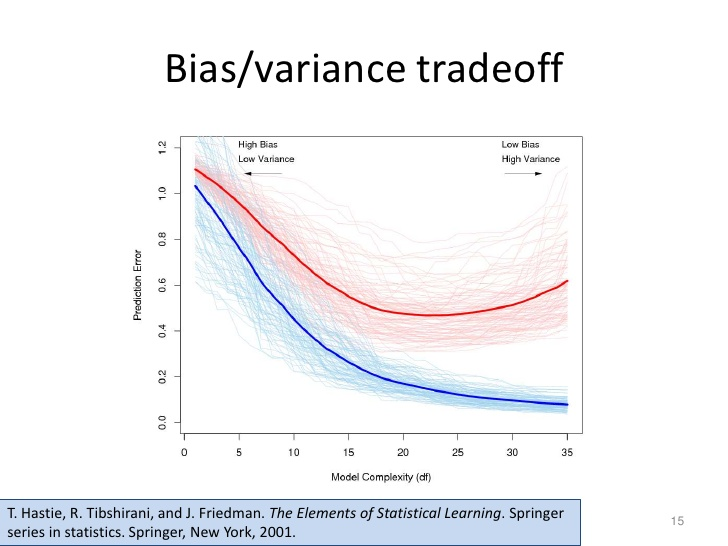
\includegraphics[width=1\textwidth]{art/support-vector-machine-15-728}
        \caption{Overfitting: 
        Prediction error on new data (red curve) versus the empirical prediction error (light blue).
        The empirical prediction error will always decrease as more complicated models are fit (moving right).
        The prediction error on new data, however, will not always decrease and will typically show a local minima.
        \label{fig:bias_variance}}
\end{figure}

Before we proceed, we now need to distinguish between several types of prediction errors.
The population \emph{risk} of a model parametrized by $\theta$, was previously defined as the average loss over all possible data instances, and denoted by $\risk(\theta)$ (\S \ref{sec:m_estimation}).
The empirical risk was defined as the average loss over the observed data points, and denoted by $\riskn(\theta)$.
We now update these definitions to deal with the the $\hyp(x)$ notation of the previous section.
\begin{align}
	\test :=& \expectg{Y,X}{\loss(Y,\hyp(X))}, \label{eq:test_error} \\
	\train :=& \expectn{\loss(y,\hyp(x))} = \frac{1}{n} \sum_i \loss(y_i,\hyp(x_i)),  \label{eq:training_error} \\
	\insample :=& \frac{1}{n} \sum_i \expectg{Y}{\loss(Y,\hyp(x_i))}, \label{eq:in_sample} \\
	\EPE :=& \expectg{\estim{\hyp}_n}{
		\expectg{Y,X}{\loss(Y,\estim{\hyp}_n(X))|\estim{\hyp}_n}
	}.\label{eq:epe}
\end{align}

Eq.(\ref{eq:test_error}) is merely a reformulation of $\risk(\theta)$ from Section~\ref{sec:m_estimation}.
It captures the expected loss, a given predictor, $\hyp(X)$, will incur on average when given new $X$'s and $Y$'s.
This will be the magnitude which will tell us which models perform well, and which do not.
It is known as the \emph{test error} or also as \emph{prediction error}.\marginnote{Test Error}

Eq.(\ref{eq:training_error}) is the reformulation of empirical risk, $\riskn(\theta)$, we have been optimizing in Section~\ref{sec:learning}.
We referred to it as the \emph{empirical risk}, but it is also known as the \emph{train error}.
\marginnote{Train Error}

Eq.(\ref{eq:in_sample}) is the average risk at the observed $x$'s, when given new $Y$'s \footnote{This magnitude should not be unfamiliar: e.g., inference in ANOVA is performed conditional on the $x$'s, which typically stem from a designed experiment.}.
This is the \emph{in sample error}.
\marginnote{In Sample Error}

Eq.(\ref{eq:epe}) is called the \emph{expected prediction error}, i.e., the expected loss when $\hyp$ is also re-learned. 
Put differently: How much would we err when:(1) we are given $n$ new examples $\sample_1$; (2) re-learn $\estim{\hyp}_n$ on $\sample_1$; (3) compute the risk of $\estim{\hyp}_n$ (in the population, not in $\sample_1$.
We emphasize this by writing $\estim{\hyp}_n$ instead of $\hyp$.
$\EPE$ is thus not a property of a particular predictor $\hyp$, but rather of a whole learning algorithm on random samples of size $n$.
It could have also been written as $\risk(algorithm)$, although I have not seen this notation in use.
\marginnote{Expected Prediction Error}


We would like to compare the performance of models based on $\test$, as this will give us an idea on the quality of the prediction on new data. 
Alas, computing $\test$ requires the distribution of $y$ and $x$, while we only have access to the $n$ observed samples.
Can the empirical risk $\train$ estimate the unknown risk $\test$? 
Figure~\ref{fig:bias_variance} suggests it cannot since $\train$ underestimates $\test$.
Why is this?
At an intuitive level: this is because with ERM we learn the $\hyp$ with smallest error in each sample.
It is thus the same as estimating the expected height in a population, by using the minimum in each sample; we will clearly be underestimating the expectation. Then again, there is the hope that we may take this minimum and debias it. 
This is the goal in the next sections.

Before proceeding, we distinguish between two similar tasks: 
\begin{description}
\item[Model Selection] This is the task of selecting between several candidate models.
\item[Model Assessment] This is the task of assessing the prediction error (i.e., the expected loss, the risk) of a given model.
\end{description}



\section{Train, Validate, Test}
\label{sec:train_test}
If data is abundant, a trivial, assumption free way to estimate $\test$\footnote{Think: why $\test$ is being estimated, and not $\EPE$ nor $\insample$?}, is to split the data into $3$ sets.
A \emph{training set}, used to learn several competing models.
A \emph{validation set}, used check the performance of the learned models and choose the best performer using some comparison measure. 
A \emph{test set}, used to estimate the risk, as the empirical risk $\train$ will be unbiased to the population risk $\test$.

If there is not enough data for this scheme, keep reading...


\section{Unbiased Estimators of the Risk}
\label{sec:risk_estimation}
Under appropriate assumptions, the bias in $\train$ when estimating $\insample$\footnote{In this case, note that it is $\insample$ being estimated, and not $\test$ nor $\EPE$.} can be computed analytically, and accounted for.
The bias $\insample-\train$ is called the \emph{optimism} of the algorithm.\marginnote{Optimism}
Akaike's Information Criterion (AIC), 
the finite sample Corrected AIC (AICc), 
Mallow's Cp (Cp), 
the Bayesian Information Criterion (BIC, aka SBC, aka SBIC), 
the Minimum Description Description Length (MDL), 
Vapnic's Structural Risk Minimization (SRM), 
the Deviance Information Criterion (DIC), 
and the Hannan-Quinn Information Criterion (HQC), 
all try to estimate $\insample$ by correcting for the optimism under different assumptions.\marginnote{Cp, AIC, BIC, MDL, SRM}

The differences, pros, and cons, of each will not be discussed herein. Just remember what they mean when you see them in your favourite software (R!).
They all have in common that you will want the model with the smallest criterion.
But be careful- as they are used for model selection, they are indifferent to scaling, and thus should be not interpreted as the expected prediction error.

\begin{remark}
Not all model selection criteria estimate $\insample$. The Focused Information Criterion (FIC), for example, does not.
\end{remark}





\paragraph{Further Reading}
For a brief review of AIC, BIC, MDL and SRM see Chapter 7 in \citep{hastie_elements_2003}. 
For a more rigorous derivation, see \cite{claeskens_model_2008}.





\section{Jackknifing}
\label{sec:jackknife}

If concerned with over fitting, here is a simple algorithm to estimate the prediction error:

\begin{algorithm}[H]
\caption{Jackknife}
\begin{algorithmic}
\For {$i \in 1,\dots,n$}
    \State $\estim{\hyp}^{(i)} \gets$ the learned model with all but the $i$'th observation.
    \State $\loss^{(i)} \gets$ the loss of $\estim{\hyp}^{(i)}$ on the $i$'th observation.
\EndFor
\State \Return the average loss over $\loss^{(i)}$.
\end{algorithmic}
\end{algorithm}

This process is called the \emph{Jackknife}, or \emph{Leave-One-Out--Cross-Validation}. 
This algorithm return an estimator of $\EPE$.
This might be quite surprising: every split uses almost an identical sample, so why would it not estimate $\test$? See Section 7.12 in \cite{hastie_elements_2003} for details..

But wait! We might be able to stabilize the variability of the estimated error in every split, if instead of leaving only a single observation aside, we leave some more. This lead to way to \emph{K-Fold Cross Validation} in the next section.


\section{Cross Validation}
\label{sec:cv}

\begin{algorithm}[H]
\caption{Cross Validation}
\begin{algorithmic}
\State Split the data into $\folds$ parts (``folds'').
\For {$\fold \in 1,\dots,\folds$}
    \State $\estim{\hyp}^{(k)} \gets$ the learned model with all \emph{except} the observations in the $\fold$'th fold.
    \State $\loss^{(\fold)} \gets$ the loss average of $\estim{\hyp}^{(\fold)}$ on the observations in the $\fold$'th fold.
\EndFor
\State \Return the average over $\loss^{(\fold)}$ .
\end{algorithmic}
\end{algorithm}

This simple algorithm estimates $\EPE$ without any assumption on the data generating process, and less data than would be required for a ``train-validate-test'' scheme.
Well, as it actually serves for model selection, it should be seen as a ``train-validate'' scheme, without the ``test'' part. It is thus \emph{not} an unbiased estimate of $\EPE$. See Section 7.12 in \cite{hastie_elements_2003} for details.

But wait again! 
The Cross Validation scheme resamples the data \emph{without replacement} to estimate $\EPE$. Could we have sampled it \emph{with} replacement? Yes. This is the idea underlying the \emph{Bootstrapping} scheme.


\section{Bootstrapping}
\label{sec:bootstrap}

Here is the simplest version of Bootstrap validation:

\begin{algorithm}[H]
\caption{Bootstrap}
\begin{algorithmic}
\For {$\bootstrap \in 1,\dots,\bootstraps$}
	\State $\sample^\bootstrap \gets$ $n$ randomly selected observations, with replacement, from the original data.
    \State $\estim{\hyp}^{\bootstrap} \gets$ the model learned with  $\sample^\bootstrap$.
    \State $\loss^{\bootstrap} \gets$ the average loss of $\estim{\hyp}^{\bootstrap}$ on the observations in the \emph{original} data.
\EndFor
\State \Return the over of $\loss^{\bootstrap}$ .
\end{algorithmic}
\end{algorithm}

This algorithm is not a good estimator of $\EPE$ as observations play a role both in learning and in validating. 
Several corrections are available. For details see Section 7.11 in \cite{hastie_elements_2003}.

The Bootstrap is a very general scheme, which can be used not only for model validation, but for assessing many of its statistical properties. It is possibly best known when used for hypothesis testing. 
For more on the Bootstrap, see \cite{efron_introduction_1994}.




% % % % % % Unsupervised % % % % %

\chapter{Unsupervised Learning}

\label{sec:unsupervised}

Unlike Supervised Learning, in Unsupervised Learning there is no outcome variable. 
There is thus no notion of ``right'' and ``wrong''. 
We merely want to learn the joint distribution of the data, $x \in \featureS$, and represent it in some way we can understand. 
Well, maybe ``merely'' is not the right word, as learning the joint distribution of the data means that instead of learning the relation between a set $x$ and another, $y$, we now try to learn the relation between all pairs of variables in $x$, which is clearly more challenging. 

Describing the data via it's joint distribution is the pinnacle, but would require many samples if $x$ has a high dimension (by high we mean $p>3$!). For higher dimensions we need to set more modest goals, which vary according to the purpose of the analysis.

The different goals of unsupervised learning can be
\begin{enumerate}
\item \textbf{Density Estimation}: Estimate $\dist(x)$.
\item \textbf{High density regions}: Find feature combinations which tend to concentrate, hopefully, because the belong to homogenous and interpretable subgroups.
\item \textbf{Low dimensional representation}: Find a low dimensional representation of the joint distribution. This allows the learning from realistic sample sizes, and analysis by, e.g., interpretable parameters and visualization.
Since this also serves in supervised learning, it is discussed with more generality in Appendix~\ref{apx:dim_reduce}.
\item \textbf{Cluster}: Assign observation to homogenous groups. In particular, the particular features of an observation are no longer of interest, once it has been assigned to a cluster.
\end{enumerate}


When thinking of machine learning the means to automate decision processes, then unsupervised learning should be seen as a per-processing stage before a supervised learning stage. Dimensionality methods in particular server to represent the data in a more compact way, thus alleviating the computational burden of supervised learning. 
Many of the methods discussed below stem from statistical literature, or signal processing literature, and were originally motivated as visualization tools. Clearly when aiming at visualization it is implied that a human is involved in the data analysis, and it is not fully automated. 

\begin{remark}[Relation to Supervised Classification]
Learning the joint data distribution, i.e., density estimation, is not only a goal for itself, but can serve for classification. 
The full data generating distribution, in the context of \emph{supervised} learning is called the \emph{generative model}.\marginnote{Generative Model}
See Appendix \ref{apx:generative_concept} for the usage of the estimated generative model for classification.
\end{remark}


\begin{remark}[Unsupervised Learning in the ERM framework]
Many unsupervised learning problems, can be cast in the ERM framework.
This has not been done in the current version of our text due to both time constraints, and compatibility with the referenced literature.
\end{remark}








\section{Cluster Analysis}
\label{sec:cluster_analysis}

In cluster analysis, we aim at assigning observations to (hopefully) homogenous and meaningful clusters. 

Groups identified are called \emph{clusters}, so that these methods are known as \emph{cluster analysis}, or \emph{data segmentation} methods.

Cluster analysis is typically easier than learning a joint distribution (\S\ref{sec:density_estimation}) or even detecting high density regions (\S\ref{sec:high_density}). 
We will see that for cluster analysis, we don't need the actual features $X$; as it will turn out, many methods only require some notion of distance between the points, and not their actual features. 
For this reason, clustering is intimately related to graph, or \emph{network}\footnote{A graph describes a yes/no relation. A network is a weighted graph, which not only describes the existence of a relation, but also its strength.} partitioning problems.



\subsection{K-Means Clustering}
\label{sec:kmeans}
The goal behind K-means clustering is finding a representative point for each of K clusters, and assign each (unlabelled) data point to one of these clusters. As each cluster has a representative point, this is also a \emph{prototype method}.\marginnote{Prototype Methods}.
The clusters are defined so that they minimize the average distance between all points to the center of the cluster.

K-means clustering requires the raw features $X$ as inputs, and not only a similarity graph. This is evident when examining Algorithm~\ref{algo:kmeans}.

In K-means, the clusters are first defined, and then similarities computed. This is thus a \emph{top-down} method.\marginnote{Top Down Clustering}

\begin{algorithm}[H]
\caption{K-Means}
\label{algo:kmeans}
\begin{algorithmic}
\State Choose the number of clusters $K$.
\State Arbitrarily assign points to clusters.
\While {Clusters keep changing}
	\State Compute the cluster centers as the average of their points.
	\State Assign each point to its closest cluster center (in Euclidean distance).
\EndWhile
\State \Return Cluster assignments and means.
\end{algorithmic}
\end{algorithm}





\subsection{K-Medoids Clustering}
\label{sec:k_medoids}


If a Euclidean distance is inappropriate for a particular $\featureS$, or that robustness to corrupt observations is required, or that we wish to constrain the cluster centers to be actual observations, then the \emph{K-Medoids} algorithm is an adaptation of K-means that allows this.

\begin{algorithm}[H]
\caption{K-Medoids}
\begin{algorithmic}
\State Choose a similarity metric $\similarity(x_i,x_j)$.
\State Choose the number of clusters $K$.
\State Arbitrarily assign points to clusters.
\While {Clusters keep changing}
	\State Within each cluster, set the center as the data point that minimizes the sum of distances to other points in the cluster.
	\State Assign each point to its closest cluster center (in $\similarity(x_i,x_j)$ distance).
\EndWhile
\State \Return Cluster assignments and centers.
\end{algorithmic}
\end{algorithm}


See Section 14.3.10 in \cite{hastie_elements_2003}.








\subsection{Hierarchical Clustering}
\label{sec:hierarchical}

These algorithms take similarity (dissimilarity) graphs as inputs.
Hierarchical clustering is a class of greedy graph-partitioning algorithms. 
Being hierarchical by design, they have the attractive property that the evolution of the clustering can be presented with a dendogram (\S\ref{sec:dendogram}).  
Unlike k-means, the method is the algorithm itself and cannot be cast as an optimization (ERM) problem.
Also, it does not require an a-priori choice of the number of cluster.

For more on hierarchical clustering see Section 14.3.12 in \cite{hastie_elements_2003}.

Two main sub-classes of algorithms can be identified: \emph{agglomerative}, and \emph{divisive}.
\subsubsection{Agglomerative Clustering}
Agglomerative clustering algorithms are bottom-up algorithm which build clusters by joining smaller clusters. 
To decide which clusters are joined at each iteration some measure of closeness between clusters is required. 
\begin{description}
\item[Single Linkage] Cluster distance is defined by the distance between the two \textbf{closest} members.
\item[Complete Linkage] Cluster distance is defined by the distance between the two \textbf{farthest} members.
\item[Group Average] Cluster distance is defined by the \textbf{average} distance between members.
\end{description}


\subsubsection{Divisive Clustering}
Divisive clustering algorithms are top-down algorithm which build clusters by splitting larger clusters. 
There are several way to divide clusters. All amount to considering some homogeneity measure on the set of all possible divisions. As this is typically computationally intense, greedy algorithms can be employed.












\subsection{Self Organizing Maps (SOM)}
\label{sec:som}
SOMs, also known as \emph{Kohonen maps}, and \emph{self organizing feature maps} (SOFM), and \emph{constrained topological map}. 
They are a dimensionality reduction method, which driven by the quality of clustering.
The method requires the original features $X$, and not only a similarity graph. \marginnote{Kohonen Map}
As such, they can be seen as the marriage of K-means clustering (\S\ref{sec:kmeans}) with dimensionality reduction (\S\ref{sec:dim_reduce_linear}).



\paragraph{Mathematics of SOMs}
[TODO]

For more on SOMs see Section 14.4 in \cite{hastie_elements_2003}. 




\subsection{Spectral Clustering}
\label{sec:spectral_clustering}

Spectral clustering is tailored for situations where \naive similarity measures $\similaritys$, such as the empirical covariances used in PCA, fail to capture the true notion of distances in the data, as it lay in some non convex set. 

For some intuition, let $X$ be $n$ images of facial expressions of the same individual. It would be quite miraculous if the Euclidean distance were to capture the true notion of distance between facial expressions. 

Spectral clustering can be decomposed into the following building blocks:
\begin{enumerate}
\item Compute the similarity graph $\similaritys$, using some \emph{local} measure of similarity.
\item Convert the similarity graph $\similaritys$ to a dissimilarity graph $\dissimilaritys$ called the \emph{graph-laplacian}.\marginnote{Graph Laplacian}
\item Embed the data in a low dimensional linear space using a spectral decomposition (\`a-la PCA) of the graph-laplacian.
\item Employ clustering techniques such as K-means (\S\ref{sec:kmeans}) on the low dimensional representation.
\end{enumerate}

The idea of using \emph{local} measures of similarity re-appears in several dimensionality reduction techniques such as LocalMDS (\S\ref{sec:localMDS}), Isomap (\S\ref{sec:isomap}) and LLE (\S\ref{sec:lle}).
Perhaps the most popular method is that of \emph{mutual K-nearest-neighbor graph}.\marginnote{Mutual K-Nearest-Neighbor Graph}

The idea of the spectral decomposition, i.e. diagonalization, of similarity measures is not a new one, and already appears in the solution to the PCA problem (\S\ref{sec:pca}). In PCA, the solution is given by using the empirical covariances as similarities. 

The idea of clustering in a low dimensional representation of the data is a powerful one. 
Spectral clustering bundles the embedding and the clustering together, but the stages can be decoupled. Any dimensionality reduction technique can be followed by a clustering technique.
SOMs (\S\ref{sec:som}) should be noted as a technique where the dimensionality reduction and the clustering \emph{cannot} be decoupled. Indeed, in SOMs, the dimensionality reduction is driven explicitly by the clustering performance.  







\section{High Density Regions}
\label{sec:high_density}

When data is high dimensional a full blown density estimation may be statistically and computationally impractical.
We can still, however, aim at detecting regions in $\featureS$ with high probability (which would have been trivial have we had a density estimate).

Once high density regions have been detected, they could be assigned to clusters. Then again, assigning to clusters is typically an easier problem which can be solved directly (see \S\ref{sec:cluster_analysis}).



\subsection{Association Rules}
\label{sec:association}
Association rules, or \emph{market basket analysis}, or \emph{affinity analysis}, can be seen as approximating the joint distribution with a region-wise constant function (Eq.~\ref{eq:decision_list}).\marginnote{Market Basket Analysis}
Put differently, we want to capture high density regions of the joint distribution of $x$ with by approximating it with a decision-list (not tree).
Learning a decision-list is a computationally impractical problem in general. Association rules are thus typically learned over binary feature spaces $\featureS$, using heuristic optimization schemes.

This type of problems typically occurs in sales analysis, where vendors seek for combinations of products that tend to sell jointly (so that can design the store better, or discount product bundles).

The \emph{Aprioiri} algorithm \cite{agraval_fast_1994}, is an example of such a heuristic search for high density combinations.\marginnote{Apriori Algorithm}






% % % Density Estimation % % % % 
\section{Density Estimation}
\label{sec:density_estimation}

We now aim at the possibly hardest target in unsupervised learning- estimating $\dist(x)$.
As previously stated, learning $\dist$ is of interest for itself, but can also serve for classification (\S\ref{sec:generative}), for detecting high density regions (\S\ref{sec:high_density}), and for clustering (\S\ref{sec:cluster_analysis}).




\subsection{Parametric Density Estimation}
If a parametric generative model can be assumed, this collapses to the parameter estimation problem in the classical statistical literature (\S\ref{sec:estimation}). Maximum Likelihood estimation being a particularly attractive approach, but certainly not the only one.
If a parametric model cannot be assumed, we fall into the realm of non-parametric methods. 
As we saw for supervised learning, these typically rely on pooling information from neighbourhoods of $\featureS$.



\subsection{Kernel Density Estimation}
\label{sec:kernel_density}

Much like the Kernel Regression regression, a \naive estimator is the moving average.
A natural generalization, in the spirit of the Nadaraya-Watson smoother (Eq.(\ref{eq:nadaraya_watson})) is the \emph{Parzen} estimate:\marginnote{Parzen Estimate}
\begin{align}
\label{eq:parzen}
	\estim{\pdf}(x):=\frac{1}{n \lambda} \sum_{i=1}^n \kernel_\lambda(x,x_i).
\end{align}

\begin{remark}
If you have been convinced by the use of KNN (\S\ref{sec:knn}) for regression (or classification), there is no reason not to use it for density estimation. It will keep offering the same pros and cons as in KNN regression (or classification).
\end{remark}

As previously stated, these methods may fail when $x$ are high dimensional. We thus recur to other methods.



\subsection{Graphical Models}
\label{sec:graphical_models}

Graphical models are graphs that represent joint distributions\footnote{Unlike \emph{graph data}, where the graph is the data itself, and not a distribution.}
For our purposes, we discuss only \emph{undirected graphical models}, also known as \emph{Markov random fields}, or \emph{Markov networks}.
The reason these models are interesting, and particularly for the purpose of density estimation, is that missing edges in a graphical model represents conditional independencies between random variables. 
If the graph structure can be assumed, and hopefully has many missing edges, then the dimension of the density estimation problem can be reduced. 

In the cases the graph structure cannot be assumed, then our goal becomes the learning of the graph structure from the data. I.e., learning the (conditional) independencies between the variables. For a multivariate Gaussian distribution, this amounts to estimating the covariance, while imposing some sparsity assumption. 
An important fact in this regard is that in the multivariate Gaussian case, missing edges in the graphical model, mean zero entries in the inverse covariance matrix. This fact sets the bridge between learning a the structure of a graphical model, and (sparse) covariance estimation.

\begin{remark}[Restricted Bolzmann Machine]
In this context it is also worth mentioning the Restricted Boltzmann Machine (RBM), which is a multivariate distribution with particular class of graphical structure, motivated from Neural Networks. \marginnote{Restricted Bolzmann Machine}
\end{remark}


For a more detailed review of Graphical Models, see Chapters 17 and 20 in \cite{wasserman_all_2004}. 















\section{Linear-Space Embeddings}
\label{sec:dim_reduce_linear}


The idea of ERM and Inductive Bias also applies to unsupervised learning.
If $\hyp(x)$ is low dimensional representation of $x$, mapping it to a ``simple'' manifold $\manifold$, we would seek some $\hyp$ that does not incur too much loss, on average. I.e., we seek to minimize $\risk(\hyp)$.

As usual, we do not have access to the data generating process of $x$, so we typically content ourselves with the empirical risk minimization.
In the context of unsupervised learing, the empirical risk is known as the \emph{reconstruction error}.\marginnote{Reconstruction Error}

The building blocks of a supervised learning problem are: 
(i) the loss function $\loss$,
(ii) the hypothesis class $\hypclass$, 
(iii) a regularization level, and
(iv) the optimization scheme.
In unsupervised learning, we have similar building blocks. We still have some loss function, regularized or not, penalizing for the poor reconstruction of the data. We can still solve an ERM problem, or replace the optimization by some other learning algorithm. The main difference is in that instead of some low dimensional mapping $\hyp:x \mapsto \estim{y}$, we learn a mapping  $\hyp:x \mapsto \estim{x}$.


For a general discussion of the idea of dimensionality reduction see Appendix~\ref{apx:dim_reduce}.

Many dimensionality reduction methods, if not all, take inspiration from the origins of PCA. It is thus strongly recommended to read the PCA section (\S\ref{sec:pca}) before proceeding.

\begin{remark}[Interpreting ``Linear'']
\label{remark:linear}
	Two interpretations of ``linear'' can be found in the literature. It may refer to the nature of the low dimensional space approximating the data, or to the nature of the embedding operation. In this text, we use the first interpretation, meaning that $\manifold$ is a linear subspace, even if the embedding operation is non linear.
\end{remark}


\begin{remark}[Dimensionality Reduction and Latent Space Generative Models]
 The methods in this section allow us to approximate the data in a lower dimension. 
 They take $X$ as inputs, and return an approximated $X$. 
 If we seek to interpret the parameters/coordinates of our data in its low dimensional representation we need to be cautious as it is probably not unique. For this purpose, see the Latent Space Generative Models Section (\S\ref{sec:latent_space}).
\end{remark}




\subsection{Principal Components Analysis (PCA)}
\label{sec:pca}

PCA is such a basic technique, it has been rediscovered and renamed independently in many fields. 
It can be found under the names of \emph{discrete Karhunen–Loève Transform; Hotteling Transform; Proper Orthogonal Decomposition (POD); Eckart–Young Theorem; Schmidt–Mirsky Theorem;  Empirical Orthogonal Functions; Empirical Eigenfunction Decomposition;  Empirical Component Analysis;  Quasi-Harmonic Modes;  Spectral Decomposition;  Empirical Modal Analysis;} and possibly more\footnote{Wikipedia: \url{http://en.wikipedia.org/wiki/Principal_component_analysis} }.
The many names are quite interesting as they offer an insight into the different problems that led to its (re)discovery.

Starting with an example, consider human height and weight data. 
While clearly two dimensional data, you don't really need both to understand how ``big'' are the people in the data. 
This is because, height and weight vary mostly along a single dimension, which can be interpreted as the ``bigness'' of an individual. 
This is why, physicians use the Body Mass Index (BMI) as an indicator of size, instead of a two-dimensional measurement.
Assume you now wish to give each individual a size score, that is a linear combination of height and weight: PCA does just that. It returns the linear combination that has the most variability, i.e., the combination which best distinguishes between individuals. 

The variance maximizing motivation above was the one that guided Hotelling \citep{hotelling_analysis_1933}.
About $30$ years before him, Karl Pearson \citep{pearson_liii._1901} derived the same procedure with a different motivation in mind. Pearson was also trying to give each individual a score. He did not care about variance maximization, however. He simply wanted a small set of coordinates in some (linear) space that approximates the original features well. As it turns out, the best linear-space approximation of $X$ is also the variance maximizing one. Pearson and Hotelling thus arrived to the same solution, with different motivations. This matter is revisited in Section 





\paragraph{Terminology}
PCA has received much attention. As such, it has rich underlying theory and terminology.
Here are some terms needed to understand PCA outputs:
\begin{itemize}
\item \textbf{Principal Components}:  The linear combinations of the features, which best separate between observations. In our example- the ``bigness'' index of each individual. The first components captures the most variance, the second components, the second most-variance, etc. In terms of $\manifold$, the principal components are an orthogonal basis for $\manifold$.
\item \textbf{Scores}: Synonymous to Principal Components.
\item \textbf{Loadings}: The weights of each data point in each principal component. In our example, the importance of the height and weight in constructing the ``bigness'' score.
\end{itemize}


\subsubsection{Intuition}
\label{sec:pca_intuition}

Notice we have currently offered two motivations for PCA: 
(i) Find linear combinations that best distinguish between observations, i.e., maximize variance. 
(ii) Find the linear subspace the bets approximates the data.
The reason these two problems are equivalent, is due to the use of the squares error.
Informally speaking, the data has some total variance. This variance can be decomposed into the part captured in $\manifold$, and the part not captured\footnote{Analogous to $SST=SSR+SSE$ in linear regression.}. 
Since the variance in the data consists of sums of squares, minimizing the distance from $X$ to $\manifold$, is the same as maximizing the variance of $X \project \manifold$, since their sum is fixed.



\subsubsection{Mathematics of PCA}
\label{sec:pca_mathematics}
We now present the derivation of PCA from the two different motivations.




\paragraph{The Variance Maximization View}
Starting with the first principal component.
If $\cov{x}=\Sigma$ then for a fixed vector $v$: $\cov{vx}=v \Sigma v'$.
Maximizing w.r.t. $v$ does not make sense as $\cov{vx}$ will explode. 
It is most convenient, mathematically, to constrain the $l_2$ norm: $\normII{v}^2=1$.
Maximizing under a constraint, using Lagrange-Multipliers: 
\begin{align}
 \argmax{v}{v \Sigma v' - \lambda (\normII{v}^2-1)}.
\end{align}
Differentiating w.r.t $v$ and equating zero: 
\begin{align}
	(\Sigma- \lambda I)v'=0
\end{align}
So the $P$ solutions for $v$ are the eigen-vectors of $\Sigma$. Which of them to pick? 
To find a \emph{global} maximum we return to the original problem, as plug our result:
\begin{align}
\label{eq:pca_maximal_variance}
 \argmax{v:\normII{v}^2=1}{v \Sigma v' }=\argmax{\lambda}{v \lambda v' }
\end{align}
so that the global maximum is obtained with the largest eigen-value $\lambda$.

Readers familiar with matrix norms will recognize that this is simply the derivation of the operator norm of $\Sigma$.

The second principal component can be found by solving the same problem, with the additional constraint of $v_2$ orthogonal to $v_1$.

The last missing ingredient is that instead of the true covariance between the features, $\Sigma$, we use the (scaled) empirical covariance $X'X$.




\paragraph{The Linear-Space Embedding View}
We now seek to find a sequence of $p$ approximations to $X$ that lay in $1,\dots,p$ dimensional linear subspaces, with respect to a least squares loss. For simplicity of exposition, we will assume that $X$ has been mean centred. 
The $\rank$'th problem to solve is thus
\begin{align}
\label{eq:pca_erm}
	\argmin{\hyp_\rank}{\normF{X-\hyp_\rank(X)}}.
\end{align}
Since $\hyp_rank$ is a map from $\reals^p$ to some rank-$\rank$ linear subspace, it must have the form $\hyp_\rank(X)=\projectMat_\rank X$ where $\projectMat_\rank$ is a $n \times n$ matrix of rank $\rank$.
Since Eq.(\ref{eq:pca_erm}) minimizes sums of (squared) Euclidean distances, $\projectMat_\rank$ has to be an orthogonal projection, thus symmetric. As such it can decomposed into an outer product $\projectMat_\rank=V_\rank V'_\rank$ where $V_\rank$ is full rank $n \times \rank$ matrix \citep[Eq.(5.13.4)]{meyer_matrix_2001}.
Under the $\rank$-space constraint, and squared error, Eq.(\ref{eq:pca_erm}) collapses to 
\begin{align}
\label{eq:pca_erm2}
	\argmin{V_\rank}{\normF{X-V_\rank V'_\rank(X)}}.
\end{align}
Using some algebraic identities \cite[Eq.(23.3)]{shalev-shwartz_understanding_2014} Eq.(\ref{eq:pca_erm2}) is equivalent to 
\begin{align}
\label{eq:pca_erm3}
	\argmax{V_\rank}{\Tr(V'_\rank XX' V_\rank)}.		
\end{align}
At this point we should note that the linear-space embedding problem has collapsed to the variance maximization problem! 
If you do not see this, just set $\rank=1$ and compare to Eq.(\ref{eq:pca_maximal_variance}), recalling that $X'X$ estimates the features' covariance $\Sigma$.






\subsubsection{PCA as a Graph Method}
\label{remark:pca_as_graph}
Starting from the maximal variance motivation, it is perhaps not surprising that PCA depends only on the similarities between features, as measured by their empirical covariance. The linearity of the target manifold was there by assumption. 

Following the linear-space embedding motivation, it is was surprising that the solutions depend only on the empirical covariances. This fact can be attributed to the use of squared error loss, which implied we were trying to decompose the total variance into the part in $\manifold_\rank$ and the orthogonal part.

From both motivations we see that the values of $X$ are of no importance given $X'X$, which can be informally thought of as a sufficient statistic\footnote{It is not a proper sufficient statistic as no generative model has been assumed.}.  

In-turn, $X'X$ depends only on the empirical covariances between \emph{individuals} ($\similaritys=XX'$), or on the Euclidean distances between individuals ($\dissimilaritys=(\norm{x_i-x_j})$).

The building blocks of all these graph-based dimensionality reduction methods are:
\begin{enumerate}
\item Compute some similarity graph $\similaritys$ (or dissimilarity graph $\dissimilaritys$) from the raw features.
\item Call upon graph embedding theory to map the data points into the target manifold $\manifold$.
\end{enumerate}
The fact that the linear-space embedding of the data depends only some similarity graph has laid a bridge between feature embedding, such as PCA, and \emph{graph embedding} methods such as MDS (\S\ref{sec:mds}).
Moreover, it has opened the door for replacing the covariance similarity, with many other similarity measures. 
Classic MDS (\S\ref{sec:mds}) is simply PCA when starting from $\similaritys$, thus viewed as a graph embedding problem.
kPCA (\S\ref{sec:kpca}) plugs kernel similarities (\S\ref{apx:rkhs}) instead of covariance similarities. 
Isomap (\S\ref{sec:isomap}), LocalMDS (\S\ref{sec:localMDS}), and LLE (\S\ref{sec:lle}) follow a similar motivation using \emph{local} measures of similarity.
Spectral Clustering (\S\ref{sec:spectral_clustering}) does some linear-space embedding \`a-la PCA, then wrapping up with a clustering algorithm in $\manifold$ \`a-la K-means. 



We now prove that the PCA solution can be cast in terms of the covariance between individuals ($\similaritys=XX'$) or the Euclidean distances ($\dissimilaritys=\norm{x_i-x_j}$).
In particular, we show that all the information on the location (mean) of $X$, needed for the PCA reconstruction, is actually encoded in $\similaritys$ (or $\dissimilaritys$).

The following exposition takes from \cite[Section 18.5.2]{hastie_elements_2003}


\paragraph{PCA with the Covariance Similarity Graph}
To begin, we need to cast the solution to the PCA problem in Eq.(\ref{eq:pca_erm3}) using the Singular Value Decomposition (SVD).\marginnote{SVD}

\begin{definition}[SVD]
Any $n \times p$ matrix $X$, can be decomposed into $X=UDV'$ where 
$U$ is an $n \times p$ orthogonal matrix ($U'U=I_p$); 
$D$ is a $p \times p$ diagonal matrix with diagonal elements $d_1 \geq d_2 \geq \dots \geq d_p$;
$V$ is a $p \times p$ orthogonal matrix ($V'V=I_p$).
\end{definition}

For mean centered $X$, the series of embeddings $\hyp_\rank(X)$ for $\rank=1,\dots,\pagebreak$ resulting from Eq.(\ref{eq:pca_erm3}) is given by $\hyp_\rank(X)=U_\rank D_\rank$, where $U_\rank$ $D_\rank$ are the $\rank$ leading columns of $U$ and $D$ respectively. $UD$ is thus the sequence of all solutions.

Now denoting $\similaritys=XX'$ and calling SVD: $\similaritys=U D^2 U'$. 
We thus see that by decomposing $\similaritys$ we can recover $U$, $D$, and thus $\hyp_\rank(X)$.

If $X$ is not mean centred, the relation still holds, but we skip the presentation.


\paragraph{PCA with the Euclidean Distance Dissimilarity Graph}
Can we convert Euclidean distances to empirical covariances? Yes!

Denote the matrix of distances of a non-centred $X$: $\dissimilaritys^2=(\norm{x_i-x_j}^2)$.
\begin{align}
	\dissimilaritys^2_{i,j} =& \norm{x_i-x_j}^2 \\
	=& \normII{x_i-\bar{x}}+\normII{x_j-\bar{x}}-2 \scalar{x_i-\bar{x}}{x_j-\bar{x}} \\
	=& \normII{x_i-\bar{x}}+\normII{x_j-\bar{x}}-2 \similaritys_{i,j}
\end{align}
where $\similaritys_{i,j}$ is the empirical covariance between individual $i$ and $j$.
We thus have 
\begin{align}
	\similaritys= - (I-M) \frac{\dissimilaritys^2}{2} (I-M)
\end{align}
where $M$ is the centring matrix: $M:= \frac{1}{n} \ones \ones'$, and $\ones$ an $n$ vector of $1$'s.




\subsection{Random Projections}
\label{sec:random_projections}

What if instead of optimizing a linear embedding of the features with respect to some criterion, such as PCA (\S\ref{sec:pca}), or FA (\S\ref{sec:factor_analysis}), we simply apply a random linear mapping $W X$. How bad will the distances between the observations be distorted? 
It turns out that not too much!
The Johnson-Lindenstrauss Lemma \citep{johnson_extensions_1984} quantifies this distortion, essentially implying that we may reduce the dimension of our data in a very \naive manner, while still conserving pair-wise similarities $\similaritys$ between observations.
 




\subsection{Sparse Principal Component Analysis (sPCA)}
\label{sec:spca}

When analyzing the PCA results, we often with to understand which features contribute to which component. 
This is much easier when the loadings, $\loadings$ are sparse, i.e., include many zeroes. 
This is the purpose of sPCA. 
We will not go into the technical detail, but merely state that sPCA performs this, \`a-la LASSO style, by means of $l_1$ regularization.







\subsection{Self Organizing Maps (SOM)}
SOMs, already discussed in Section~\ref{sec:som}, are a linear-subspace dimensionality reduction method, aimed at good clustering. 


\subsection{Multidimensional Scaling (MDS)}
\label{sec:mds}

MDS aims at representing a network\footnote{The term Graph is typically used in this context instead of Network. But a graph allows only yes/no relations, while a network, which is a weighted graph, allows a continous measure of similarity (or dissimilarity). It is thus more appropriate.} of distances (or similarities) between observations, by embedding the observations in a $\rank$ dimensional \emph{linear} subspace, while preserving the original distances.
The network may be obtained by computing some similarity (or dissimilarity) measure with the raw features $X$, or simply because the data itself is a network (social, communication, etc.).

Since MDS mainly serves for visualizing data, it is most natural to use $\rank=2$. 
The embedding will distort the original distances (or\dots), and may even change the ordering of the observations. The good news is that it is easier to visualize \andor cluster them in their new simplified representation. 

If the input of MDS is the empirical covariance similarity network, then MDS with ``classical scaling'' (see below) returns the exact same solution as PCA.

The embedding is merely the assigning of each point to a location in some lower dimensional linear space $\manifold$. 
The assignment is driven by a \emph{stress function} which penalizes for the average distortion created by the embedding.
The different types of MDSs, such as \emph{Classical MDS}, and \emph{Sammon Mappings}, differ in the stress function driving the embedding.

For more on MDS see Section 14.8 in \cite{hastie_elements_2003} or \cite{borg_modern_2005}.


\paragraph{Mathematics of MDS}
We start with either a dissimilarity network $\dissimilaritys=(\dissimilarity_{i,j})$, or a similarity network $\similaritys=(\similarity_{i,j})$.
Similarities can be thought of as correlations, and dissimilarities as distances (which are indeed the typical measures in use).
Define $z_i \in \reals^\rank$ the location of point $i$ in the target linear space of rank $\rank$. 
The $z_i$'s are set to minimize some penalty for geometric deformation called the \emph{stress function}.
Typical stress functions include:
\begin{description}

\item[Classical MDS] Using the centred inner product (i.e. empirical covariance) as the similarity measure and minimizes the squared distortion:
$\similarity_{i,j}:= \scalar{x_i-\bar x}{x_j-\bar{x}}$ and the new location are given by
\begin{align}
\label{eq:mds_classical}
	 \argmin{z_1,\dots,z_n}{\sum_{i,j=1}^{n} (\similarity_{i,j}-\scalar{z_i-\bar z}{z_j-\bar{z}} )^2}.
\end{align}

\item[Least Squares] Also known as \emph{Kruskal-Shepard}. Also minimizes the squared distortion. 
\begin{align}
\label{eq:mds_stress}
	 \argmin{z_1,\dots,z_n}{\sum_{i \neq j} (\dissimilarity_{i,j}-\norm{z_i-z_j} )^2}.
\end{align}

\item[Sammon Mapping] Also known as \emph{Sammon's stress}, aims at minimizing the \emph{proportion} of distortion:
\begin{align}
\label{eq:mds_sammon}
	 \argmin{z_1,\dots,z_n}{\sum_{i \neq j} \frac{(\dissimilarity_{i,j}-\norm{z_i-z_j} )^2}{\dissimilarity_{i,j}}}.
\end{align}

\end{description}


\begin{remark}[Classical and Least Squares MDS]
Although they both minimize the squared distortion, working with $\similaritys$ or $\dissimilaritys$ lead to different solutions. 
In particular, Classical is a linear embedding while Stress is not. 
\end{remark}




\subsection{Local MDS}
\label{sec:localMDS}
Local MDS is motivated by the observation that if the data does not lay in a globally convex subspace, then global distances are a very distorted measure, whereas geodesic distances should be used instead. 
Their solution is to compute $\dissimilaritys$ using only local distances, and then calling upon MDS.

\begin{remark}[The Non-Linearity of Local MDS]
\label{remark:linearity_of_localMDS}
Local MDS is typically considered a non-linear-space embedding, thus belonging to Section \ref{sec:dim_reduce_nonlinear}.
I currently do not think is the case, as it is presented as a linear space embedding.
Maybe Remark \ref{remark:nldr} can explain the confusion in terminology.
\end{remark}



\subsection{Isometric Feature Mapping (Isomap)}
\label{sec:isomap}

Isomap, also known as \emph{principal coordinate analysis}, is another method intimately related to MDS(\S\ref{sec:mds}).\marginnote{Principal Coordinate Analysis}

Isomap follows the same motivation as Local MDS (\S\ref{sec:localMDS}), but with a different algorithm to compute the dissimilarity matrix $\dissimilaritys$.

\begin{remark}[The Non-Linearity of Isomap]
Just like Local MDS, Isomap is typically considered a non-linear-space embedding (see Remark \ref{remark:linearity_of_localMDS}).
I currently do not think is the case.
\end{remark}









% % % % Non linear dimensionality reduction % % % % %
\section{Non-Linear-Space Embeddings}
\label{sec:dim_reduce_nonlinear}


Section \ref{sec:dim_reduce_linear} deals with representing the data in a \emph{linear} sub space $\manifold$. They all aim at finding a basis which efficiently represents that data, with respect to some target function. 
In this section, we allow $\manifold$ to be non-linear. 
We will thus no longer be able to represent the data by its coordinates in some basis.


\begin{remark}[Non Linear Dimensionality Reduction]
\label{remark:nldr}
	Do not let the title of this section be confused with the term Non-Linear Dimensionality-Reduction (NLDR).
	NLDR deals with the nature of the \emph{embedding} operation, and not with the structure of the target manifold $\manifold$ (see also Remark \ref{remark:linear}).\marginnote{NLDR}
	This section deals with embeddings into a non-linear subspace, regardless of the nature of the embedding operator.
	Cases of non-linear embeddings (NLDR) into a \emph{linear} manifolds $\manifold$ belong in Section~\ref{sec:dim_reduce_linear}.
\end{remark}




\subsection{Kernel Principal Component Analysis (kPCA)}
\label{sec:kpca}

Back to the motivating example from the PCA section (\S\ref{sec:pca}): assume we want to construct a ``bigness'' score, that best separates between individuals, but we no longer constrain it to be a linear function of the height and weight.
Recalling that the best discrimination between observations means maximizing the variance of the \emph{scores} given to individuals, we could try to find the best separating score $g(x)$ by solving 
\begin{align}
\label{eq:kpca_wrong}
	\argmax{g}{\covn{g(X)}}
\end{align}
where $g(x)$ maps an individual's features to a score in $\manifold$.

Alas, just like in the supervised learning problem, without any constraints on $\manifold$, thus on $g$, we might overfit \andor not be able to compute $g$ as optimization is done in a infinite dimensional space. 
We thus have two matters to attend:
(i) We need to constrain $g(x)$ so that it does not overfit.
(ii) We need the problem to be computable.
This is precisely the goal of kPCA. 

We have already encountered a similar problem with Smoothing Splines (\S\ref{sec:smoothing_splines}). It is thus not surprising that the solution has the same form. 
Namely, if we choose the right $g$'s, the solution of Eq.(\ref{eq:kpca_wrong}) takes a very simple form. 
The classes of such $g$'s are known as Reproducing Kernel Hilbert Spaces (RKHS). 
They are discussed in Appendix~\ref{apx:rkhs}.



\paragraph{Mathematics of kPCA}
[TODO]



\subsection{Principal Curves}
[TODO]



\subsection{Local Linear Embedding (LLE)}
\label{sec:lle}

LLE aims at finding linear subspaces that are good approximations of small neighbourhoods of the whole data $X$.
It is similar in spirit to Isomap (\S\ref{sec:isomap}) and LocalMDS (\S\ref{sec:localMDS}).
It differs, however, in the way similarities are computed, and in the way embeddings are performed. 
In particular, as the name may suggest, LLE performs local embeddings to linear subspaces. The resulting approximating manifold $\manifold$, being the ``stitching'' of many linear spaces, is ultimately non linear.




\subsection{Information Bottleneck}
[TODO]

%The \emph{information bottleneck} is an information theoretic framework, due to \cite{tishby_information_1999}, that generalizes the idea of dimensionality reduction and data compression.
%It is a general statement of the problem of maximal compression of $X$, while preserving as much of the information in $X$ as possible.
%To state the general problem we require some definitions from information theory.
%
%\begin{definition}[Entropy]
%The entropy of a random variable $\x$ is defined as the expected negative log density of $\x$: 
%$$\expect{-\log \pdf(\x)}.$$
%\end{definition}
%
%\begin{definition}[Mutual Information]
%The mutual information between two random variable $\x$ and $\y$ is defined as : 
%$$\expect{\log \frac{\pdf(\x,\y)}{\pdf(\x) \pdf(\y)}}.$$
%\end{definition}
%
%Informally speaking, the entropy is a measure of the variability of a distribution, and the mutual information is a measure of deviation from independence, i.e., captures the amount of information $\x$ carries on $\y$, and vice-versa.
%With this intuition, and denoting the compression of $x$ by $y=g(x)$, we may define the compression problem as:
%\begin{align}
%	\argmin{g}{arg2}
%\end{align}


\begin{remark}[Information Bottleneck and ICA]
[TODO]
\end{remark}





%%%%%%%%% Generative Models %%%%%%%%%%%



\section{Latent Space Generative Models}
\label{sec:latent_space}

We have already met generative models for supervised learning (\S\ref{sec:generative}), and for unsupervised learning (\S\ref{sec:density_estimation}).
We now discuss a class of generative models, that can be seen as a dimensionality reduction device. 
The following models and methods assume that the data generating process is governed by some low dimensional unobservable \emph{state}, also known as \emph{latent variable}, or \emph{hidden variable}.
This is why these models are also known as \emph{state space} models. A term coined by  \citet{kalman_contributions_1960}.\marginnote{State-Space Models}

The simplification of the generative model from its original high-dimension allows us to:
(i) \emph{Interpret} the data generating process via its states. 
(ii) \emph{Formulate} the density estimation problem as a low dimensional problem, we can actually hope to solve, even when the data itself is very high dimensional.
(iii) \emph{Visualize} the data. 

The fundamental idea is that while the data generating distribution may have a complicated form, when we condition on the unobserved variable, the distribution greatly simplifies. 



\subsection{Factor Analysis (FA)}
\label{sec:factor_analysis}

Factor Analysis is solved very similarly to PCA (\S\ref{sec:pca}), so that the two are often confused. 
FA, however, stems from a rather different motivation than PCA.
PCA is motivated by finding variable combinations (scores) with most variance. 
FA is a generative method, aimed at finding uncorrelated latent attributes. 

In FA we assume that the observed $X$'s depend linearly on a set of $\rank$ independent latent (i.e. unobservable) attributes we denote with $\latent$.
The generative model is thus
\begin{align}
\label{eq:factor}
	X=\loadings \latent+\varepsilon
\end{align}
Assuming a generative distribution on $\latent$ and $\varepsilon$, we may try to estimate $\loadings \latent$ by maximum likelihood.
Recovering the particular latent attributes $\latent$ from $\estim{\loadings\latent}$ is still impossible as there are infinitely many such solutions. To see this, consider an orthogonal \emph{rotation} matrix $\rotation$ ($\rotation' \rotation=I$). For each such $\rotation$: $ \loadings \latent=\loadings \rotation' \rotation \latent = \loadings^* \latent^*$.

The choice of $\rotation$ changes the interpretation of the latent attributes. This is why many researchers find FA an unsatisfactory inference tool.

\begin{remark}[Identifiability in PCA]
	The non-uniqueness (non-identifiability) of the FA solution under variable rotation is never mentioned in the PCA context. Why is this?
	This is because the methods have different purposes. 
	Generative latent variables, as in FA, are only defined up to rotations. They are thus not unique. 
	Combinations with maximal variance, as in PCA, are unique. There is no room for rotations.
\end{remark}



\paragraph{FA Terminology}
\begin{itemize}
\item \textbf{Factors}: The unobserved attributes $\latent$. Not to be confused with the \emph{principal components} in the context of PCA.
\item \textbf{Loadings}: The $\loadings$ matrix; the contribution of each attribute to the observed $X$.
\item \textbf{Rotation}: An orthogonal re-combination of the latent attributes $\latent$ and loadings, which changes the interpretation of the result.
\end{itemize}


For a brief review of Factor Analysis see \cite{hastie_elements_2003}.
For an full exposition, and a discussion of the differences with PCA, see \cite{jolliffe_principal_2002}.




\subsection{Independent Component Analysis (ICA)}
\label{sec:ica}

ICA is a family of latent space models as it assumes data is generated as some function of the latent variables $\latent$. 
In many cases this function is assumed to be linear in $\latent$ so that ICA is compared, if not confused, with PCA or FA. 

The fundamental idea of ICA is that $\latent$ has a joint distribution of \emph{independent} variables. 
This is a stronger assumption that the typical FA assumption where the distribution of $\latent$ is merely assumed to be uncorrelated. 
This independence assumption solves the the non-uniquness of the latent attributes in FA (\S\ref{sec:factor_analysis}).

Two assumptions distinguish ICA from FA, allowing the identification of $\latent$: 
(i) The latent variables are \textbf{not} Gaussian distributed.
(ii) The latent variables are statistically \emph{independent}.

Being a generative model, estimation of $\latent$ can then be done using maximum likelihood, or an information theoretic criterion called \emph{infomax}.\marginnote{Infomax}



ICA is a popular technique in signal processing, where $\latent$ is actually the signal (e.g. sound) produced by several different sources. 
Recovering $\latent$ is thus recovering the original signals mixing in the recorded $X$. This is known as \emph{blind source separation}.\marginnote{Blind Source Seperation}


\begin{remark}[ICA and FA]
The solutions to the (linear) ICA problem can ultimately be seen as a solution to the FA problem with a particular rotation $\rotation$ implied by the independence assumption.
Put differently, the formulation of the (linear) ICA problem, implies a unique rotation. 
\end{remark}

For a general discussion of ICA see \cite{jolliffe_principal_2002}.
For a brief exposition of the linear ICA see \cite{hastie_elements_2003}. 
For a detailed review of ICA see \cite{hyvarinen_independent_2000}. 



\paragraph{Mathematics of ICA}
[TODO]








\subsection{Exploratory Projection Pursuit}
\label{sec:exploratpory_ppr}
[TODO]




\subsection{Compressed Sensing}
\label{sec:compressed_sensing}
[TODO]





\subsection{Generative Topographic Map (GTM)}
\label{sec:gtm}
[TODO]



\subsection{Mixtures}
A very simply, perhaps the simplest, class of latent variable generative models, is that of Finite Mixtures. 
In a finite mixture, the fundamental assumption is that the observed data is sampled from $K$ unobserved classes. Each class, having some simple joint distribution. 
Being unobserved, we cannot directly learn the conditional simple distributions, without somehow learning the class assignments. 
The likelihood function of such data, is thus the \emph{marginal} probability over all possible classes, thus a \emph{mixture}.
The good news is that a very complex generative model, may be much more easy to learn and interpret if we can assume, or approximately assume, it is actually a finite mixture.

The probability density of a mixture of $K$ classes, each with density $\pdf_k(x)$, is given by  
\begin{align}
\label{eq:mixture}
	\pdf(x)=\sum_{k=1}^{K} \pi_k \pdf_k(x)
\end{align}
where $\pi_k$ is the probability of class $k$.



\begin{remark}[Finite Mixture Distributions]
While very simple to understand, mixture distributions are an unpleasant probabilistic creature. 
Because the probability mass (or density) function is additive in the underlying mixing components, is has a very challenging functional form.
For instance- the likelihood problem with be non-convex with multiple local extrema, so that numerical optimization schemes are not guaranteed to converge.
It may also be the case that the likelihood is unbounded, so that the local extrema are not a global extrema, complicating our attempts at maximum likelihood estimation. 
Hypothesis testing for the number of mixing components is also very challenging as classical statistical theory assumptions do not apply.
\end{remark}


\begin{remark}[Mixtures And the Expectation Maximization Algorithm (EM)]
As previously stated, the likelihood function of mixtures is typically non convex. 
It's optimization is typically done with a numerical algorithm called the Expectation Maximization (EM) algorithm.
Roughly speaking, the idea behind the EM, is that in each iteration observations are assigned to classes, the simple conditional distributions learned, then reasigned using the learnt parameters, etc.\ until convergence.
Even though convergence to an optimum is not guaranteed, it is by far the most popular framework for learning mixtures.
\end{remark}



\begin{remark}[Mixtures For Clustering]
Because the output of learning a mixture, is a density like Eq.(\ref{eq:mixture}), a learnt mixture can easily serve for clustering by a simple application of Bayes rule. Simple assign an observation to the cluster with highest (posterior) probability:
\begin{align}
\label{eq:mixture_posterior}
	\prob{x \in k|x}=\frac{\pi_k \pdf_k(x)}{\pdf(x)}
\end{align}
\end{remark}



\begin{remark}[Mixture in Supervise Learning]
The generative models underlying several supervised learning methods, are actually finite mixtures.
Fisher's LDA (\S\ref{sec:lda}) implies a finite mixture of Gaussians, with the same covariance and different means.
Fisher's QDA (\S\ref{sec:qda}) implies a finite mixture of Gaussian, with different covariance and different means.
\Naive Bayes (\S\ref{sec:naive_bayes}) implies a mixture of some distribution, with independent components.
\end{remark}





\subsection{Hidden Markov Models (HMM)}
\label{sec:hmm}
Hidden Markov Models may have two possible interpretations.

The first, and perhaps most common, is as a generalization of the mixture model in the case the generative model assumes dependencies between $x_i$'s and we wish to use a mixture model. 
In this case, we need to model and learn the transition probabilities between states (or classes, are we previously referred to the hidden states of a mixture). 
Assuming the transition between states follows a \emph{Markov process}, i.e., the probabilities of transition depends only upon the current state, the resulting model is an \emph{hidden Markov model}, or \emph{hidden Markov chain}.
\marginnote{Markov Process}

The second, is as a generalization of the Graphical Models (\S\ref{sec:graphical_models}). 
This generalization is known a \emph{latent space graphical model} (\S\ref{sec:latent_graphical}). 
In this case, the Markov property does not describe the process of transition between states, but rather a property of the conditional distribution in each state ($\pdf_k(x)$). 




\subsection{Latent Space Graphical Models}
\label{sec:latent_graphical}

The idea of simplifying a complicated distribution by conditioning on some latent variable can be compounded with the idea of a graphical model (\S\ref{sec:graphical_models}). 
Put differently, the generative model can be a simple graphical model when conditioned on some latent variable.
We do not pursue this avenue further, and refer the reader to Section 17.4.2 in \cite{hastie_elements_2003}.





\subsection{Matrix Factorization}
\label{sec:matrix_factorization}
[TODO]




% % % % Random Graphs % % % % %
\section{Random Graph Models}
\label{sec:random_graphs}

There are several occasions in which our date does not consist of the classical features $X$, but rather directly given as a similarity (dissimilarity) graph. This can happen when the data itself is a graph, such as social networks, communication networks, protein interactions networks, etc. It may also be the case that the original data is indeed given as features, which was used to compute a similarity (dissimilarity) graph. Indeed, We have already seen that for the purpose of clustering, we only need some proximity graph between observations, and not the whole features. 

Random Graphs are a class of \emph{generative models}, but unlike other generative methods, the model does not specify a distribution over the features, but rather a distribution over the proximity measures.
For this, it is  intimately related to \emph{random graph} and \emph{random matrix} theory.

For a review of random graph models see \cite{goldenberg_survey_2010}.


\subsection{\erdos \renyi}
[TODO]

\subsection{Exchangeable Graph Model}
[TODO]

\subsection{$p1$ Graph Model}
[TODO]

\subsection{$p2$ Graph Model}
[TODO]

\subsection{Stochastic Block Graph Model}
[TODO]

\subsection{Latent Space Graph Model}
[TODO]

\subsection{Exponential Random Graphs (ERGMs)}
[TODO]

\begin{remark}[Relation to Spectral Clustering]
[TODO]
\end{remark}






% % % % % % Collaborative Filtering % % % % %
\chapter{Recommender Systems and Collaborative Filtering}
\label{sec:collaborative_filtering}


% % % % recommender systems % % % % % % %
\section{Recommender Systems}

A recommender system is a software that, as the name suggests, gives recommendations to the user. 
Notable examples include Book recommendations by Amazon, and film recommendations by Netflix.
The two main approaches to recommender systems include \emph{content filtering} and \emph{collaborative filtering}.



% % % % Content filtering % % % % % %
\section{Content Filtering}

In content filtering, the system is assume to have some backround information on the user (say, because he logged in), and uses
this information to give him recommendations.
The recommendation in this case, is approached as a supervised learning problem: 
the system learns to predict a product's rating ($y$) based on the user's features ($x$).
It then computes the rating for many candidate products and recommends a set with high predicted ratings.



% % % % colaborative filtering % % % % %
\section{Collaborative Filtering}

Unlike content filtering, in \emph{collaborative filtering}, there is no external information on the user or the products, besides the ratings of other users. 
The term collaborative filtering, was coined by the authors of the first such system-- Tapestry \citep{goldberg_using_1992}. 

Collaborative filtering can be approached as a supervised learning problem, or as an unsupervised learning problem. This is because it is neither. 
It is essentially a \emph{missing data} problem.\marginnote{Missing Data}
To see this consider a matrix of rankings, $\rankings$ where the $i,j$'th entry, $\ranking_{i,j}$, is the ranking of user $i$ movie $j$. 
Predicting $\ranking_{i,j'}$, i.e., the ranking of a currently unseen movie, is essentially an imputation of a missing value.


The two main approaches to collaborative filtering include \emph{neighbourhood methods}, and \emph{latent factor models} \cite{koren_matrix_2009}.

\subsubsection{Neighbourhood Methods}
The neighbourhood methods to collaborative filtering rest on the assumption that similar individuals have similar tastes. 
If someone similar to individual $i$ has seen movie $j'$, then $i$ should have a similar opinion.

The notion of using the neighbourhood of a data point is not a new one. We have seen it being used for supervised learning in kernel regression (\S\ref{sec:kernel}) and KNN (\S\ref{sec:knn}).

Neighbourhood methods for collaborative filtering, or missing data imputation in general, can thus be seen as supervised learning problems, and solved in the same way.


\begin{remark}[Collaborative Filtering and Other Supervised Learning Methods]
If you are wondering, why only neighbourhood methods for supervised learning apply to collaborative filtering, you are right.
Any supervised learning method can be applied to impute entries in $\rankings$. Neighbourhood 
methods are merely the most popular.
\end{remark}


\subsubsection{Latent Factor Models}
The latent factor approach to collaborative filtering rests on the assumption that the rankings are a function of some latent user attributes and latent movie attributes. 
This idea is not a new one, as we have seen it in the context of unsupervised learning in factor analysis (FA) (\S\ref{sec:factor_analysis}), independent component analysis (ICA) (\S\ref{sec:ica}), and other latent space generative models.
From the relation between FA and PCA, it should also come as no surprise that collaborative filtering can also be viewed as a matrix approximation problem. 
When approximating the rankings matrix ($\rankings$) with some simple manifold $\manifold$, en-passant, we also impute the missing entries in $\rankings$.

We now see that collaborative filtering, and missing data imputation in general, can also be approached as an unsupervised learning problem. 



\section{The Relation Between Supervised and Unsupervised Learning}
It may be surprising that collaborative filtering can be seen as both an unsupervised and a supervised learning problem.
But these are not mutually exclusive problems. 
In fact, the relation has already been implied in the introduction to the unsupervised learning section (\S\ref{sec:unsupervised}), and we now make it explicit.

In unsupervised learning we try to learn the joint distribution of $x$, i.e., try to learn the relationship between any variable in $x$ to the rest, we may see it as several supervised learning problems. In each, a different variable in $x$ plays the role of $y$. 

Many unsupervised learning methods can be seen in this light. We, however, will not be exploring this avenue right now.




% % % % % % Appendices % % % % % %
\newpage

\appendix


% % % % % % RKHS % % % % %

\chapter{The Kernel Trick and Reproducing Kernel Hilbert Spaces (RKHS)}
\label{apx:rkhs}

In the context of supervised learning the \emph{kernel trick} is a mathematical device that allows to learn very complicated predictors ($\hyp$) in a computationally efficient manner. 
More generally, in the context of unsupervised learning, the kernel tricks allow to learn complicated non-linear mappings of the original features (and not only predictor functions). 

Not all predictors and not all problem admit this trick. Then again, many do. 
Methods for which it applies include:
SVM's (\S\ref{sec:svm}), principal components analysis (\S\ref{sec:pca}), canonical correlation analysis (\S\ref{sec:cca}), ridge regression (\S\ref{sec:ridge}), spectral clustering (\S\ref{sec:spectral_clustering}), Gaussian processes\footnote{See the Bayesian interpretation below to see why they apply to Gaussian Processes.}, and more\footnote{This partial list is taken from Wikipedia: \url{http://en.wikipedia.org/wiki/Kernel_method}}.

We now give an exposition of the method in the context of supervised learning. 


Think of smoothing splines (\S\ref{sec:smoothing_splines});
It was quite magical that without constraining the hypothesis class $\hypclass$, the ERM problem in Eq.(\ref{eq:smoothing_spline}) has a finite dimensional closed form solution.
The property of an infinite dimensional problem having a solution in a finite dimensional space is known as the \emph{kernel property}.\marginnote{Kernel Property}
We with to generalize this observation and ask- which problems have the kernel property?
Stating the general optimization problem:
\begin{align}
\label{eq:rkhs}
	\argmin{\hyp}{\frac{1}{n} \sum_i \loss(y_i,\hyp(x_i)) + \lambda J(\hyp) }
\end{align}
The problem is then- what type of penalties $J(\hyp)$ will return simple solutions to Eq.(\ref{eq:rkhs}).
The answer is: function that belong to \emph{Reproducing Kernel Hilbert Space} function spaces. 
RKHS's are denoted by $\rkhs$.
They include many functions, but they are a rather ``small'' subset of the space of all possible functions.
These spaces, and the functions therein, are defined by another function called a \emph{Kernel} denoted by $\kernel$. 
Choosing a particular kernel defines the space and the functions therein.
Choosing a particular kernel, also defines the form of $J$ in Eq.(\ref{eq:rkhs}).
Put differently: for any choice of a kernel $\kernel$, there is a particular $J(\hyp)$ for which the solution of Eq.(\ref{eq:rkhs}) will be a function in $\rkhs$ and will be easily computable. 


\section{Mathematics of RKHS}
We now show how choosing a kernel $\kernel$ defines a space $\rkhs$, and a penalty $J(\hyp)$.

A kernel is a non-negative symmetric function of two arguments: $\kernel(x,y): \reals^p \times \reals^p \mapsto \reals_+$.
By fixing $y$, $\kernel(x,y)$ is a function with a single argument $x \mapsto \kernel(x,y)$.
$\rkhs$ is merely the space of functions of $x$, spanned at given $y$'s: 
\begin{align}
\label{eq:rkhs_span}
	\hyp(x):\sum_m \al_m \kernel(x,y_m)
\end{align} 

From linear algebra, you may know that positive definite matrices be diagonalized. 
This analogy carries to $\kernel$, which admits an eigen-expansion: 
\begin{align}
\label{eq:rkhs_eigen}
	\kernel(x,y)=\sum_{i=1}^\infty \gamma_i \phi(x) \phi(y)
\end{align}
Using Eqs.(\ref{eq:rkhs_eigen}) and (\ref{eq:rkhs_span}) we can thus expand elements $f$ of $\rkhs$: 
\begin{align}
	\hyp(x)=\sum_{i=1}^\infty c_i \phi(x)
\end{align}
where $c_i=\gamma_i \sum_m \alpha_m \phi(y)$.
We also define a norm $\normrkhs{\hyp}^2$ in this space, which is induced by $\kernel$:
\begin{align}
\label{eq:rkhs_norm}
	\normrkhs{\hyp}^2 := \sum_{i=1}^\infty \frac{c_i^2}{\gamma_i}
\end{align}

The penalty $J(\hyp)$ in Eq.(\ref{eq:rkhs}), is simply be $\normrkhs{\hyp}^2$.
The $\hyp$'s that solve Eq.(\ref{eq:rkhs}) are guaranteed to have a simple form. They reside in an $n$ dimensional linear function space \citep{wahba_spline_1990}:
\begin{align}
	\hyp(x)=\sum_{i=1}^n \al_i \kernel(x,x_i)
\end{align}

The functions $\kernel(x,x_i)$ can be seen as a basis to the solution space. 
The good news continue! Being only $n$ dimensional, the norms of these $\hyp$'s, do not require integration but rather only finite summation:
\begin{align}
	\normrkhs{\hyp}^2=\sum_{i=1}^n \sum_{j=1}^n \kernel(x_i,x_j) \al_i \al_{j} := \al' K \al.
\end{align}

Adding the above results, we can restate Eq.(\ref{eq:rkhs}) and say that when fixing $\kernel$ and using the appropriate $J$, we only need to solve: 
\begin{align}	
\label{eq:rkhs_simple}
		\argmin{\al}{\frac{1}{n} \sum_i \loss(y_i-K_i \alpha) + \lambda \al' K \al }
\end{align}
which is a quadratic programming problem over an $n$ dimensional linear space, easily solvable with numeric routines.


\section{The Bayesian View of RKHS}
Just as the ridge regression (\S\ref{sec:ridge}) has a Bayesian interpretation, so does the kernel trick.
Informally, the functions solving Eq.(\ref{eq:rkhs}) can be seen as the posterior mode if our prior beliefs postulate that the function we are trying to recover is a Gaussian zero-mean process with covariance given by $\kernel$.
This view suggests the intuition that the regularization introduced by $J(\hyp)$ shrinks the estimated $\hyp$ towards a smoother function. At an extreme, where $\lambda\to\infty$, we will recover a constant function, since the the mode of our Gaussian process prior is at the origin of $\rkhs$.


\section{Kernel Generalization of Other Methods}
[TODO: Sec 18.5.2]

% % % % % % % % Generative models % % % % % % % %

\chapter{Generative Models}
\label{apx:generative_concept}

By \emph{generative model} we mean that we specify the whole data distribution. This is particularly relevant to supervised learning where many methods only assume the distribution of $\dist(y|x)$ without stating the distribution of $\dist(x)$.
Assuming only $\dist(y|x)$ is known as a \emph{discriminative model}, or \emph{discriminative analysis}.\marginnote{Descriminative Model}
In a generative model, in contrast, we assume the whole $\dist(y,x)$.

For the mere purpose of making a prediction, we do not need to learn $\dist(y,x)$. 
Knowing this distribution, however, does permit to make predictions, via Bayes Theorem: 
$\dist(y|x)=\frac{\dist(y,x)}{\int\dist(y,x)dy}$.
Generative models make use of this relation to make predictions. 

To gain some intuition, consider a supervised learning problem where the data has an equal number of samples per class. 
Learning the distribution of $x$ withing each class, allows to a simple classification of a given $x$ to the class with highest probability. LDA (\S\ref{sec:lda}), QDA (\S\ref{sec:lda}), and \Naive Bayes (\S\ref{sec:naive_bayes}) follow this exact same rational.




% % % % % % % % % Dimensionality Reduction % % % % % % %

\chapter{Dimensionality Reduction}
\label{apx:dim_reduce}

Dimensionality reduction is a useful concept in both supervised and unsupervised learning. 
It allows to represent high dimensional data in a lower dimension. This allows the visualization of the data in a human-tractable dimension, the application of low-dimensional algorithms, and the reduction of computational burden when using the data for supervised learning. 

The fundamental idea behind dimensionality reduction is that while $\featureS$ may be high dimensional, thus $\dist(x)$ hard to learn, there is hope that $\x$ does not really vary in the whole space. 
If the mass of $\dist(x)$ is concentrated around some low dimensional manifold $\manifold$, then the original problem might be approximated to learning the distribution of the projection $\dist(X \project \manifold)$ on $\manifold$. 
If $\manifold$ is fairly low dimensional, we may hope to visualize and understand $\dist(X \project \manifold)$ with fairly simple tools.
Dimensionality reduction also reduces the memory required to represent the data. It is thus intimately related to \emph{lossy compression} in information theory.\marginnote{Lossy Compression}

A similar reasoning justifies dimensionality reduction in supervised learning. 
While $\dist(x)$ might vary in the whole $\featureS$, but there might be only few directions which carry information on $y$. Learning $\dist(y|x)$ can thus be well approximated by $\dist(y|x \project \manifold)$.

As was first observed in the context of PCA (\S\ref{sec:pca}), for many types of embeddings, i.e., for many target manifolds and reconstruction errors, we do not really need the original data $X$, but rather only a graph of similarities (or dissimilarities) between data points. 
As we see in the unsupervised learning section (\S\ref{sec:unsupervised}), many dimensionality reduction techniques stem from the \emph{graph mebedding} and \emph{graph drawing} literature. As such, they only require similarity (dissimilarity) matrices as inputs. 


\begin{remark}
The subspace $\manifold$, which approximates $\dist(x)$ may differ than the one that approximates $\dist(y|x)$. Despite this, it is still quite common for a supervised learning problem to be preceded by an unsupervised dimensionality reduction stage.
\end{remark}


\section{Graph Drawing}
[TODO]





% % % % % % % % % Information Theory % % % % % % %

\chapter{Information Theory}
\label{apx:information_theory}


\begin{definition}[Entropy]
\label{def:entropy}
[TODO]
\end{definition}



\begin{definition}[Mutual Information]
\label{def:mutual_information}
[TODO]
\end{definition}



\begin{definition}[Kullback–Leibler Divergence]
\label{def:kl_divergence}
[TODO]
\end{definition}





% % % % % % Notation % % % % %


\chapter{Notation}
\label{apx:notation}

In this text we use the following notation conventions:
\begin{description}
\item[$\ones$] A vector of $1$'s.
\item[$x$] A scalar or vector.
\item[$\x$] A (possibly) vector valued random variable.
\item[$X$] A matrix.
\item[$\x$]  A matrix valued random variable (a random matrix).
\item[$X'$] The matrix transpose of $X$.
\item[$\normII{x}$] The $l_2$ norm of $x$: $\sqrt{\sum_j x_j^2}$.
\item[$\normI{x}$] The $l_1$ norm of $x$: $\sum_j |x_j|$
\item[$\normF{X}$] The Frobenius matrix norm of X: $\normF{X}^2=\sum_{ij} x_{ij}^2$
\item[$\ortho{n}$] The space of orthogonal matrices. 
\item[$\scalar x y$] The scalar product of two vectors $x$ and $y$.
\item[$\sample$] A data sample.
\item[$\expect{\x}$] The expectation of $\x$.
\item[$\expectn{x}$] The empirical expectation (average) of the vector $x$.
\item[$\cov{\x}$] The covariance matrix of $\x$: $\expect{(\x-\expect{\x})(\x-\expect{\x})'}$.
\item[$\covn{x}$] The empirical covariance matrix of x: $\expectn{(x-\expectn{x})(x-\expectn{x})'}$.
\item[$\rho(\x,\y)$] The correlation coefficient.
\item[$\cdf{x}{t}$] The CDF of $\x$ at $t$.
\item[$\icdf{x}{\al}$] The inverse CDF at $\al$ (the quantile function).
\item[$\cdfn{x}{t}$] The empirical CDF of data vector $x$.
\item[$\icdfn{x}{\al}$] The empirical $\al$ quantile of the data vector $x$.
\item[$\x \sim \dist$]  The random variable $\x$ is $\dist$ distributed. 
\item[$\pdf(x)$] The density function of $\dist$ at $x$.
\item[$\gauss{\mu,\sigma^2}$] The univariate Gaussian distribution with mean $\mu$ and variance $\sigma^2$.
\item[$\gauss{\mu,\Sigma}$] The multivariate Gaussian distribution with mean vector $\mu$ and covariance matrix $\Sigma$.
\item[$\lik(\theta)$] The likelihood function at $\theta$.
\item[$\loglik(\theta)$] The log likelihood function at $\theta$.
\item[$\loss(x,\theta)$] The loss function of $\theta$ at $x$.
\item[$\risk(\theta)$]  The risk at $\theta$.
\item[$\riskn(\theta)$] The empirical risk at $\theta$.
\item[$\hyp(x)$] A prediction (hypothesis) at $x$.
\item[$\hypclass$] The class of all hypotheses $\hyp$.
\item[$\plane$] A hyperplane.
\item[$\categories$] A set of categories. 
\item[$\positive{t}$] The positive part of $t$.
\item[$\kernel(x,y)$] A kernel function evaluated at $(x,y)$.
\item[$\indicator{A}$] The indicator function of the set $A$.
\item[$\manifold$] A manifold.
\item[$\project$] A projection operator.

\item[$\similarity_{ij}$] A similarity measure between observations $i$ and $j$. 
\item[$\dissimilarity_{ij}$] A dissimilarity measure between observations $i$ and $j$. 
\item[$\similaritys$] A weighted graph (network), i.e. matrix, of similarities between observations. 
\item[$\dissimilaritys$] A weighted graph (network), i.e. matrix, of dissimilarities between observations. 

\item[$\kl{\x}{\y}$] Kullbeck-Leibler divergence between random variable $\x$ to $\y$.
\item[$\entropy(\x)$] The entropy of random variable $\x$.
\item[$\mutual{\x}{\y}$] The mutual information between $\x$ and $\y$.


\end{description}







%%%%%%%%% Bibliography %%%%%%%%%%%
\newpage
\addcontentsline{toc}{chapter}{Bibliography}
\bibliographystyle{abbrvnat}
\bibliography{Intro2MachineLearning}


\end{document}